
\chapter{Background Knowledge}
\label{cha:background}

\section{Controller Area Network}
\label{sec:can}
Controller Area Network (CAN) is a serial two-wire bus specified as Classical CAN in the Bosch CAN specification \cite{BoschCAN}
and extended in the CAN FD specification \cite{BoschCANFD}.
One wire is the CAN High (CAN H), the other CAN Low (CAN L).
The bus can either be in the recessive state, which is seen as a logical one, or in the dominant state, which is seen as logical zero.
The so-called "wired-AND" structure enforces a dominant bit to override a recessive bit.
For transmitting a recessive bit, the bus is in the idle state, where both lines are at the same voltage level.
For writing a dominant bit, the CAN H wire is tied to the positive voltage supply, and the CAN L wire is tied to a low level.
\autoref{fig:can_level} shows this principle.
CAN use a Non-Return-to-Zero Coding (NRZ), which means that the level at the bus is held for the entire bit time.
A bit stuffing mechanism provides reliable synchronization for the time of the frame transmission.
The idle level for both wires should be kept at a constant level about half the supply level.
However, the physical layer is neither fully specified by the Bosch CAN specification \cite{BoschCAN} \cite{BoschCANFD}
nor the ISO CAN specification \cite{ISO11898} and is left to the system integrator.

\begin{figure}[htp]
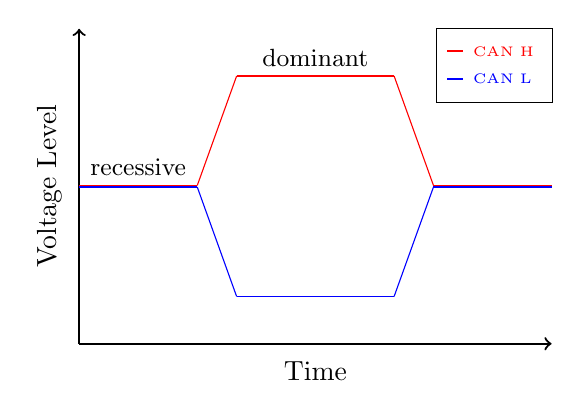
\begin{tikzpicture}
	%Draw axis
	\draw[thick,->] (0,0) -- coordinate (x axis mid) (6,0);
	\draw[thick,->] (0,0) -- coordinate (y axis mid) (0,4);
	%Draw axis label
	\node[below=0.1cm] at (x axis mid) {Time};
	\node[rotate=90, above=0.1cm] at (y axis mid) {Voltage Level};
	%Draw legend
	\matrix [draw,below left] at (current bounding box.north east) {
  		\draw[thick, red]  (0,0) -- (0.2,0) {} node[right]{\tiny CAN H}; \\
  		\draw[thick, blue] (0,0) -- (0.2,0){} node[right]{\tiny CAN L}; \\
	};

	%Draw CAN H
	\draw[red] (0,2.01)   -- (1.5,2.01) node[black, midway, above]{\small recessive};
	\draw[red] (1.5,2.01) -- (2,3.4);
	\draw[red] (2,3.4)    -- (4,3.4)    node[black, midway, above]{\small dominant};
	\draw[red] (4,3.4)    -- (4.5,2.01);
	\draw[red] (4.5,2.01) -- (6,2.01);
	%Draw CAN L
	\draw[blue] (0,1.99) -- (1.5,1.99);
	\draw[blue] (1.5,1.99) -- (2,0.6);
	\draw[blue] (2,0.6)    -- (4,0.6);
	\draw[blue] (4,0.6)    -- (4.5,1.99);
	\draw[blue] (4.5,1.99) -- (6,1.99);

	%
\end{tikzpicture}
\caption{CAN Physical Bit Transmission}
\label{fig:can_level}
\end{figure}

\subsection{Wiring and Bus Access}
\label{sec:wiring_access}

For wiring, a two-wire twisted pair cable with an impedance of 120$\Omega$ is used.
The topology is a line topology where stubs are allowed, but with a maximum length, depending on the bus speed.
On the first and last node of the bus line, terminating resistors with a value 120$\Omega$ avoid reflections on the bus line.
An example with two nodes is shown in \autoref{fig:can_wiring}.

\input{figures/can_wiring}

A CAN-transceiver, like shown in \autoref{fig:can_transceiver} connects the controller to the bus.
This transceiver converts the logic-level signals from the controller (CAN RX and CAN TX) to the bus levels and vice versa.
The dominant timeout protects the bus from a persistent dominant state in case of a faulty CAN controller.

\begin{figure}[htp]
\begin{circuitikz} \draw
	(4.5,3) node[op amp, rotate=180] (amp){}
	(amp.+) to [short,-o] ++(4, 0) node[right] {CAN H}
	(amp.-) to [short,-o] ++(4, 0) node[right] {CAN L}
	(2,3) node[invschmitt, rotate=180] (schm){}
	(amp.out) to (schm.in)
	(schm.out) to [short,-o] ++(-1, 0) node[left] {CAN RX}
	(8,5) node[pmos,emptycircle] (pmos){}
	(8,1) node[nmos] (nmos){}
	(8,0.5) node[ground] (gnd){}
	(8,6) node[vss, rotate = 180] (vss){}
	(pmos.S) to (vss)
	%(pmos.G) to [short] ++(-0.5,0)
	(pmos.D) to [short,-*] ++(0,-0.75)
	(nmos.D) to [short,-*] ++(0,0.75)
	(2.75,4.75)node[draw, minimum height=1cm, minimum width=2cm] (timeout) {\small Dominant Timeout}
	(5.75,4.75) node[draw, minimum height=1cm, minimum width=1.5cm] (driver) {\small Driver}
	(6.5,5) to (pmos.G)
	(6.5,4.5) to (7,4.5) to (7,1) to (nmos.G)
	(timeout) to (driver)
	(1,4.75) to [short,-o] ++(-0.75,0) node [left] {CAN TX}
	;
\end{circuitikz}
\caption{Simplified CAN Transceiver}
\label{fig:can_transceiver}
\end{figure}

The bitrate limit depends on the length of the bus \cite{TiCANPhy}.
However, the highest bitrate is limited to 1 Mbit per second for Classical CAN \cite{BoschCAN} and 8 Mbit for the data field of CAN Flexible Data-Rate (CAN FD)\cite{BoschCANFD}.
\autoref{tab:bus_speed} shows some example length and bitrate combinations for Classical CAN.
For CAN FD, the bitrate is only increased during the data field phase and could be eight times higher than the values in the table.

\begin{table}[ht]
	\centering
	\caption{Maximum bus speed}
	\begin{tabular}{|c|c|} 
		\hline
		Length & Max. Speed \\ \hline
		[m]    & [Kbps]     \\
		\hline
		\hline
		40     & 1000       \\ \hline
		100    & 500        \\ \hline
		200    & 250        \\ \hline
		500    & 100        \\ \hline
		1000   & 50         \\ \hline
	\end{tabular}
	\label{tab:bus_speed}
\end{table}

\FloatBarrier

\subsection{CAN Frames}
\label{sec:can_frames}

\begin{figure}[htp]
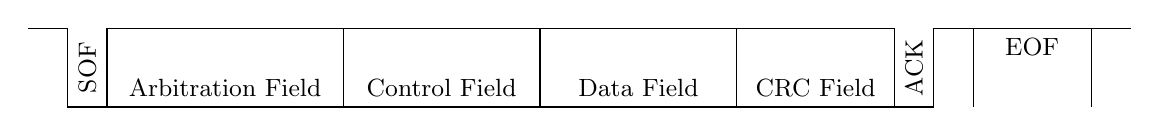
\begin{tikzpicture}
	%SOF
	\draw (0,1) -- ++(0.5,0) -- ++(0,-1) -- ++(0.5,0) -- ++(0,1);
	\node[rotate=90] at (0.75,0.5) {\small SOF};
	%Arbitration Field
	\draw (1,1) -- ++(3, 0);
	\draw (1,0) -- ++(3, 0) node[midway, above=0.25] {\small Arbitration Field};
	\draw (4, 0) -- ++(0,1);
	%Control Field
	\draw (4,1) -- ++(2.5, 0);
	\draw (4,0) -- ++(2.5, 0) node[midway, above=0.25] {\small Control Field};
	\draw (6.5, 0) -- ++(0,1);
	%Data Field
	\draw (6.5,1) -- ++(2.5, 0);
	\draw (6.5,0) -- ++(2.5, 0) node[midway, above=0.25] {\small Data Field};
	\draw (9, 0) -- ++(0,1);
	%CRC Field
	\draw (9,1) -- ++(2, 0);
	\draw (9,0) -- ++(2, 0) node[midway, above=0.25] {\small CRC Field};
	\draw (11, 0) -- ++(0,1);
	%ACK Field
	\draw (11,0) -- ++(0.5,0);
	\draw (11.5,0) -- ++(0,1);
	\node[rotate=90] at (11.25,0.5) {\small ACK};
	\draw (11.5,1) -- ++(0.5,0);
	\draw (12,0) -- ++(0,1);
	%EOF
	\draw (12,1) -- ++(1.5, 0) node[midway, below=0.25] {\small EOF};
	\draw (13.5, 0) -- ++(0,1);
	\draw (13.5,1) -- ++(0.5,0);

\end{tikzpicture}
\caption{CAN Frame Format}
\label{fig:can_frame_format}
\end{figure}

The Medium Access Control (MAC) specification defines the CAN frame format, as shown in \autoref{fig:can_frame_format}.
CAN uses so-called identifiers to identify the frames. Identifiers do not address nodes but identify the data that is being sent.
There are four basic frame formats. The "CAN Base Frame Format" with an 11-bit identifier; the "CAN Extended Frame Format" with a 29-bit identifier and their FD variants.
Frames start with the "Start of Frame" (SOF) bit. This bit is always dominant and signalizes the start of the frame and synchronizes the nodes.
The Arbitration Field includes the Base identifier and the "Remote Transmission Request" (RTR) bit in case of a basic frame.
For the extended frame format, the Identifier Extension (IDE) bit signalizes the identifier extension.
In this case, the IDE-bit and the remaining 18 bits of the identifier are also part of the Arbitration Field.
Nodes can use the RTR-bit to signal other nodes a request for transmission. For example, trigger a sensor read.

\begin{figure}[htp]
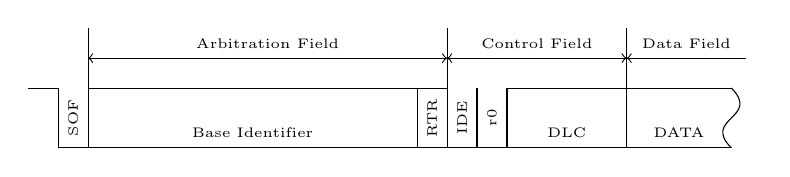
\begin{tikzpicture}[scale=0.76]
	%SOF
	\draw (0,1) -- ++(0.5,0) -- ++(0,-1) -- ++(0.5,0) -- ++(0,1);
	\node[rotate=90] at (0.75,0.5) {\tiny SOF};
	%Base Identifier
	\draw (1,1) -- ++(5.5, 0);
	\draw (1,0) -- ++(5.5, 0) node[midway, above=0.25] {\tiny Base Identifier};
	\draw (6.5, 0) -- ++(0,1);
	%RTR
	\draw (6.5, 0) -- ++(0.5,0);
	\draw (6.5, 1) -- ++(0.5,0);
	\draw (7, 0) -- ++(0,1);
	\node[rotate=90] at (6.75,0.5) {\tiny RTR};
	%IDE
	\draw (7, 0) -- ++(0.5,0);
	\draw (7.5, 0) -- ++(0,1);
	\node[rotate=90] at (7.25,0.5) {\tiny IDE};
	%r0
	\draw (7.5, 0) -- ++(0.5,0);
	\draw (8, 0) -- ++(0,1);
	\node[rotate=90] at (7.75,0.5) {\tiny r0};
	%DLC
	\draw (8,1) -- ++(2,0);
	\draw (8,0) -- ++(2,0) node[midway, above=0.25] {\tiny DLC};
	\draw (10, 0) -- ++(0,1);
	%data
	\draw (10,1) -- ++(1.75,0);
	\draw (10,0) -- ++(1.75,0) node[midway, above=0.25] {\tiny DATA};
	\draw (11.75,0) .. controls (11.25,0.5) and (12.25,0.5) .. (11.75,1);

	%Arbitration
	\draw (1,1) -- ++(0,1);
	\draw (7,1) -- ++(0,1);
	\draw[<->] (1,1.5) -- (7,1.5) node[midway, above] {\tiny Arbitration Field};
	%Control
	\draw (10,1) -- ++(0,1);
	\draw[<->] (7,1.5) -- (10,1.5) node[midway, above] {\tiny Control Field};
	%Data
	\draw[<-] (10,1.5) -- (12,1.5) node[midway, above] {\tiny Data Field};

\end{tikzpicture}
\caption{CAN Base Frame}
\label{fig:can_std_frame}
\end{figure}
\begin{figure}[htp]
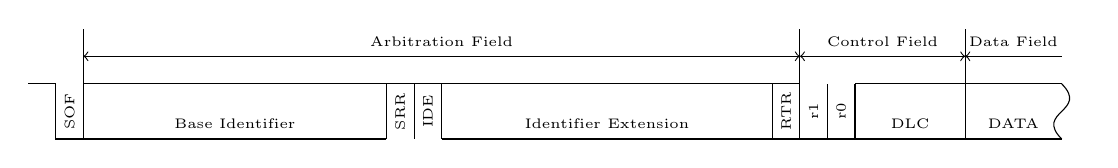
\begin{tikzpicture}[scale=0.7]
	%SOF
	\draw (0,1) -- ++(0.5,0) -- ++(0,-1) -- ++(0.5,0) -- ++(0,1);
	\node[rotate=90] at (0.75,0.5) {\tiny SOF};
	%Base Identifier
	\draw (1,1) -- ++(5.5, 0);
	\draw (1,0) -- ++(5.5, 0) node[midway, above=0.25] {\tiny Base Identifier};
	\draw (6.5, 0) -- ++(0,1);
	%SRR
	\draw (6.5, 1) -- ++(0.5,0);
	\draw (7, 0) -- ++(0,1);
	\node[rotate=90] at (6.75,0.5) {\tiny SRR};
	%IDE
	\draw (7, 1) -- ++(0.5,0);
	\draw (7.5, 0) -- ++(0,1);
	\node[rotate=90] at (7.25,0.5) {\tiny IDE};
	%Identifier Extension
	\draw (7.5,1) -- ++(6, 0);
	\draw (7.5,0) -- ++(6, 0) node[midway, above=0.25] {\tiny Identifier Extension};
	\draw (13.5, 0) -- ++(0,1);
	%RTR
	\draw (13.5,0) -- ++(0.5,0);
	\draw (13.5,1) -- ++(0.5,0);
	\draw (14,0) -- ++(0,1);
	\node[rotate=90] at (13.75,0.5) {\tiny RTR};
	%R1 R0
	\draw (14,0) -- ++(1,0);
	\draw (14.5,0) -- ++(0,1);
	\node[rotate=90] at (14.25,0.5) {\tiny r1};
	\draw (15,0) -- ++(0,1);
	\node[rotate=90] at (14.75,0.5) {\tiny r0};
	%DLC
	\draw (15,1) -- ++(2,0);
	\draw (15,0) -- ++(2,0) node[midway, above=0.25] {\tiny DLC};
	\draw (17, 0) -- ++(0,1);
	%Data
	\draw (17,1) -- ++(1.75,0);
	\draw (17,0) -- ++(1.75,0) node[midway, above=0.25] {\tiny DATA};
	\draw (18.75,0) .. controls (18.25,0.5) and (19.25,0.5) .. (18.75,1);
	
	%Arbitration
	\draw (1,1) -- ++(0,1);
	\draw (14,1) -- ++(0,1);
	\draw[<->] (1,1.5) -- (14,1.5) node[midway, above] {\tiny Arbitration Field};
	%Control
	\draw (17,1) -- ++(0,1);
	\draw[<->] (14,1.5) -- (17,1.5) node[midway, above] {\tiny Control Field};
	%Data
	\draw[<-] (17,1.5) -- ++(1.75,0) node[midway, above] {\tiny Data Field};
	
	\end{tikzpicture}
	\caption{CAN Extended Frame}
	\label{fig:can_ext_frame}
\end{figure}

\autoref{fig:can_std_frame} and \autoref{fig:can_ext_frame} shows examples for a Basic and Extended Frames.
CAN FD frames are outlined in more detail in the Bosch CAN FD specification \cite{BoschCANFD}.

In the Arbitration Field, collisions of multiple sending nodes are allowed.
The fact that a dominant bit always overrides a recessive bit resolves collisions in a way that the frame with the lowest identifier always wins.
Senders that want to write a recessive bit but get overridden by a dominant bit must abort their transmission silently.
Aborted frames can be retransmitted when the bus is in the idle state again.

The Control Field includes the reserved bit r0, the IDE, and the Data Length Code (DLC) for Basic frames and reserved bit r1, r0, and the DLC for Extended frames.
DLC indicates how many bytes are transmitted during the data phase.
\autoref{tab:dlc} lists the codes and number of bytes.
The maximum number of bytes for Classical CAN frames is eight, and the maximum number of bytes for CAN FD is 64.

\begin{table}
	\centering
	\caption{Data Length Codes}
	\begin{tabular}{|c|c|} 
		\hline
		DLC & Bytes \\
		\hline
		\hline
		0-8 & 0-8 \\ \hline
		9   & 12  \\ \hline
		10  & 16  \\ \hline
		11  & 20  \\ \hline
		12  & 24  \\ \hline
		13  & 32  \\ \hline
		14  & 48  \\ \hline
		15  & 64  \\ \hline
	\end{tabular}
	\label{tab:dlc}
\end{table}

The data field can be either empty or as many bytes as indicated by the DLC.

After the data field, the CRC field follows.
The length of the CRC field depends on the length of the data field.
A 15-bit CRC is used for all CAN frames up to eight data bytes.
For data field length up to 16 bytes, a 17-bit CRC is used.
A 21-bit CRC is used for a data field length of more than 16 bytes.
The CRC is calculated over the whole frame, from SOF to the end of the data field.

All nodes that received the frame correctly acknowledge their reception by putting a dominant bit into the ACK field.
The Field after the ACK field is the ACK-Delimiter and is always recessive.

EOF is the "End Of Frame". It is always seven recessive bits.
The Inter Frame Space is at least three recessive bits called Intermission.
Any node can override this Intermission with dominant bits to signal an Overload condition.

\begin{figure}[htp]
	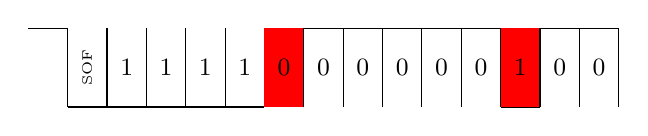
\begin{tikzpicture}[scale=1]
		\draw (0,1) -- ++(0.5,0);
		\foreach \x in {0.5,1,...,2.5}{
			\draw (\x,0) -- ++(0,1);
			\draw (\x,0) -- ++(0.5,0);
		}

		\node[rotate=90] at (0.75,0.5) {\tiny SOF};

		\foreach \x in {1,1.5,...,2.5}{
			\node[minimum height=1cm, minimum width=0.5cm] at (\x + 0.25,0.5) {\small 1};
		}

		%stuffing 1
		\draw (3,0) -- ++(0,1);
		\draw (3,1) -- ++(0.5,0);
		\node[fill=red, minimum height=1cm, minimum width=0.5cm] at (3.25,0.5) {\small 0};
		
		\foreach \x in {3.5,4,...,5.5}{
			\draw (\x,0) -- ++(0,1);
			\draw (\x,1) -- ++(0.5,0);
			\node[minimum height=1cm, minimum width=0.5cm] at (\x + 0.25,0.5) {\small 0};
		}
		
		%stuffing 2
		\draw (6,0) -- ++(0,1);
		\draw (6,0) -- ++(0.5,0);
		\node[fill=red, minimum height=1cm, minimum width=0.5cm] at (6.25,0.5) {\small 1};

		\foreach \x in {6.5,7}{
			\draw (\x,0) -- ++(0,1);
			\draw (\x,1) -- ++(0.5,0);
			\node[minimum height=1cm, minimum width=0.5cm] at (\x + 0.25,0.5) {\small 0};
		}
		\draw (7.5,0) -- ++(0,1);

	\end{tikzpicture}
	\caption{Bit Stuffing Example for 0x780 Identifier}
	\label{fig:can_stuffing}
\end{figure}

The bit-stuffing mechanism provides reliable synchronization during the transmission of the frame.
Five consecutive bits of the same value force a so-called stuffing bit.
The stuffing bit is a bit with the inverted value of the bits before and must be ignored by the receivers.
Stuffing bits change the length of the frame. An example is shown in \autoref{fig:can_stuffing}.
In the example stuffing bits, highlighted in red, extends the identifier field to 13 bits.
Additionally, it shows that SOF must be taken into account for stuffing.

Intentional violations of the stuffing rule are called Error Frames.
Overriding six consecutive bits with a dominant bit is an Error Active Frame.
Six recessive bits are called Error passive frame.
This rule allows signaling error conditions during all phases, including the EOF, in case of a CRC mismatch.

\FloatBarrier

\section{ISO-TP Transport Protocol}
\label{sec:iso_tp}

ISO-TP is a short name for the transport protocol specified in ISO15765 \cite{ISO15765}.
It specifies a transport protocol and network layer service operating in Controller Area Networks.
It was initially designed for road vehicle diagnostic services but it is not limited to them.
ISO-TP overcomes the limited frame size of CAN frames and allows us to send packets up to 4095 bytes and in the latest version extended to 4 gigabytes.
For this, the packets are segmented, transmitted in CAN frames, and reassembled on the receiver.
Additionally, a flow-control mechanism is defined to steer the timing of the frames.

The header data is called Process Control Information (PCI). The first nibble is the PCI-Type.
Following four PCI types are defined:
\begin{itemize}
	\item Single Frame
	\item First Frame
	\item Consecutive Frame
	\item Flow Control Frame
\end{itemize}

The rest of the PCI depends on the PCI-Type.
After the PCI, the rest of the frame is filled with payload data.
Single frames are used when the payload data plus one byte for the PCI  fits into a single CAN frame.
For Classical CAN, it is a payload length of seven bytes. For CAN FD, it can be up to 63 bytes.
The other three PCI types are used for payload lengths larger than a single frame can carry.

A segmented packet starts with a "First Frame" (FF) from the sender to the receiver.
The First Frame contains information about the total payload data length.
The receiver sends back a "Flow Control" frame (FC).
This FC frame can either signal "Continue To Send", "Wait", or that the packet would "Overflow" the receiver.
Furthermore, the FC frame contains a Block Size (BS) and Minimal Separation Time (ST\textsubscript{min}).
When the FC frame is of type CTS, the sender continues with sending "Consecutive Frames" (CF).
When BS is zero, the sender sends as many CF frames as needed to transfer the payload data.
Otherwise, the sender has to stop after BS CF frames and wait for another FC frame.
ST\textsubscript{min} defines a minimum separation time between two frames.
A ST\textsubscript{min} of zero is allowed.
If the receiver answers with an FC-Frame with the Flow-State OVFLW, the sender has to abort the transmission.
In case the sender does not receive an FC-Frame within one second, it aborts the transmission.
The Flow-State WAIT causes a reset of the sender timeout.
Receivers cancel the reception of the packet when no CF frame is received within one second.

\autoref{fig:iso_tp_sequence} shows an example sequence with a BS of three.

\input{figures/iso_tp_sequence.tex}

\begin{table}
	\centering
	\caption{ISO-TP Protocol Control Information}
	\begin{tabular}{|c|c|c|c|c|c|c|c|c|c|} \hline
	Byte:                 & \multicolumn{2}{c|}{0}              & \multirow{2}{*}{1}  & \multirow{2}{*}{2} & \multirow{2}{*}{3} & \multirow{2}{*}{4} & \multirow{2}{*}{5} & \multirow{2}{*}{6} & \multirow{2}{*}{7} \\ \cline{2-3}
	                      & 7..4               & 3..0           &                     &                    &                    &                    &                    &                    &                    \\ \hline \hline
	\multirow{2}{*}{SF}   & \multirow{2}{*}{0} & SF\_DL         & data 0              & data 1             & data 2             & data 3             & data 4             & data5              & data 6             \\ \cline{3-10}
	                      &                    & 0              & SF\_DL              & data 0             & data 1             & data 2             & data 3             & data 4             & data 5             \\ \hline
	\multirow{2}{*}{FF}   & \multirow{2}{*}{1} & \multicolumn{2}{c|}{FF\_DL}          & data 0             & data 1             & data 2             & data 3             & data 4             & data 5             \\ \cline{3-10}
	                      &                    & \multicolumn{2}{c|}{0}               & \multicolumn{4}{c|}{FF\_DL}                                                       & data 0             & data 1             \\ \hline
	CF                    & 2                  & SN             & data 0              & data 1             & data 2             & data 3             & data 4             & data 5             & data 6             \\ \hline
	FC                    & 3                  & FS             & BS                  & STmin              & \multicolumn{5}{c|}{}                                                                                  \\ \hline
	\end{tabular}
	\label{tab:pci}
\end{table}

\begin{table}
	\centering
	\caption{Flow-States}
	\begin{tabular}{|l|c|} \hline
	Type  & Number \\ \hline \hline
	CTS   (Continue To Send)  & 0      \\ \hline
	WAIT  (Wait)              & 1      \\ \hline
	OVFLW (Overflow)          & 2      \\ \hline
	\end{tabular}
	\label{tab:fs}
\end{table}

\autoref{tab:pci} shows examples of classical CAN frames with all PCI types.
Elements labeled with data 0 to data 6 are payload data.

\newpage

SF is the Single Frame and has the PCI-type-number 0.
For Single Frames with maximum payload data size of seven bytes, the Single Frame data length (SF\_DL) is encoded in bit zero to three of the first PCI byte.
CAN FD frames can have a frame data length up to 64 bytes in a single frame. Single frames with more than seven bytes of data encode the data length in the second PCI byte.

FF is the First Frame and has the PCI-type-number 1.
The data length (FF\_DL) of the packet is encoded in byte zero and byte one of the PCI.
Byte one is the lower octet, and bit zero to bit 3 of byte 0 contains the upper nibble of the 12-bit data length.
For a data length bigger than 4095 bytes, bit zero to three of byte zero and byte one is set to zero.
The data length is then encoded in byte two to five.

CFs are Consecutive Frames, containing payload data and a sequence number (SN).
The PCI-type-number is 2, and the sequence number is located at the lower nibble of byte zero.
The sequence number is a counter that is set to one for the first CF and incremented by one for every frame and wraps around at 15.
When the sequence number wraps around, it starts with zero again.
The sequence number is used to detect out of order or lost frames.

FCs are Frame Control Frames and have the PCI-type-number 3.
The lower 4-bit nibble of the first byte contains Flow State. The numbers are shown in \autoref{tab:fs}.
The second byte, Block-Size (BS), defines how many CF frames the sender is allowed to transmit until he has to wait for an FC-Frame again.

\FloatBarrier

\section{IPv6}
\label{sec:ipv6}

\begin{table}
	\centering
	\caption{Internet Protocol Suite}
	\begin{tabular}{|c|l|l|} \hline
	Layer                         & Example                      \\ \hline \hline
	Application                   & HTTP, HTTPS, CoAP, MQTT      \\ \hline
	Transport                     & TCP, UDP                     \\ \hline
	\cellcolor{black!10} Internet & IPv4, IPv6, ICMP             \\ \hline
	Link                          & Ethernet, IEEE 802.15.4, CAN \\ \hline
	\end{tabular}
	\label{tab:ips}
\end{table}

IP (Internet Protocol) covers the Internet layer of the Internet Protocol Suite (\autoref{tab:ips}) \cite{rfc1122}.
Internet Protocol version six (IPv6) was first introduced in RFC2460 \cite{rfc2460} as an RFC Draft-Standard in December 1998
and got finally standardized with RFC8200 \cite{rfc8200} in July 2017.
It solves some problems from its predecessor, the Internet Protocol version four (IPv4) \cite{rfc791}.

The most significant improvements are:

\begin{itemize}
	\item Extended address range (from 32 bits to 128-bits)
	\item Stateless Address Autoconfiguration
	\item Simplification of the header
	\item Use of Neighbor Discovery protocol
	\item Next header instead of header options
\end{itemize}

RFC8200 defines some important terminologies:
A "node" is a device with an IPv6 stack.
"Link" refers to the lowest layer defined in \autoref{tab:ips}, and
"interface" is the node's attachment to a link.

\subsection{IPv6 Addresses}
\label{sec:ipv6_addr}

IPv6 addresses are written in a hexadecimal representation of 16-bit blocks, separated by colons.
Leading zeros can be omitted, and all zero blocks can be written as two colons (::).
The all-zero blocks can span more than a single 16-bit block, but can only be used once in a representation.
RFC5952 \cite{rfc5952} describes the recommended text representation of IPv6 addresses.

For example, the address fe80:0000:0000:0000:0000:00ff:fe00:1234 can be written as fe80::ff:fe00:1234

An IPv6 address prefix can be written as \textit{IPv6-address/prefix-length}.
For example fe80::00ff:fe00:1234/64 is interpreted as fe80:000:0000:0000 address prefix.

\begin{table}
	\centering
	\caption{IPv6 Address Types}
	\begin{tabular}{|l|l|l|} \hline
	Type                & Prefix            \\ \hline \hline
	Unspecified Address & ::/128 (all zero) \\ \hline
	Loopback            & ::1/128           \\ \hline
	Multicast           & FF00::/8          \\ \hline
	Link-Local Unicast  & FE80::/10         \\ \hline
	Global Unicast      & everything else   \\ \hline
	\end{tabular}
	\label{tab:ipv6_addr_types}
\end{table}

RFC4291 \cite{rfc4291} defines five types of addresses, identified by their higher-order bits.
The address types are shown in \autoref{tab:ipv6_addr_types}.

\begin{figure}[htp]
	\begin{center}
	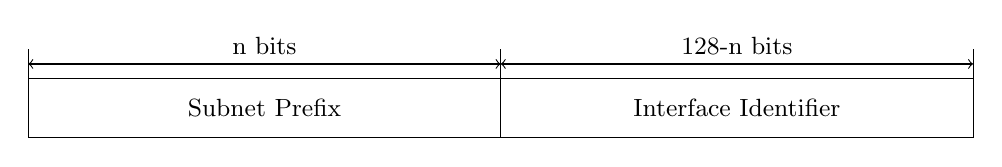
\begin{tikzpicture}[scale=0.75]
		\draw (0,0) rectangle (16,1);
		\draw (0,1) -- ++(0,0.5);
		\draw (8,0) -- ++(0,1.5);
		\draw (16,1) -- ++(0,0.5);
		\node at (4, 0.5) {\small Subnet Prefix};
		\node at (12, 0.5) {\small Interface Identifier};
		\draw[<->] (0,1.25) -- (8,1.25) node[midway, above] {\small n bits};
		\draw[<->] (8,1.25) -- (16,1.25) node[midway, above] {\small 128-n bits};
	\end{tikzpicture}
	\end{center}
	\caption{Subnet Prefix of an IPv6 address}
	\label{fig:ipv6_subnet_prefix}
\end{figure}

Unicast IPv6 addresses can generally be treated as if they have no internal structure.
Nevertheless, more sophisticated nodes may be aware of subnets, which logically group addresses.
\autoref{fig:ipv6_subnet_prefix} shows how the address is split into the subnet prefix and an Interface Identifier (IID).
Routers, for example, can use subnets to create hierarchical boundaries.
The IID needs to be unique within the subnet and identifies an interface on a link (lowest layer on \autoref{tab:ips}).
All Unicast addresses not starting with the binary value 000 must have an IID according to the Modified EUI-64 format with a length of 64 bits.
Addresses of this format can be derived from the link-address as described in RFC4291 \cite{rfc4291} Appendix A.
If the address is derived, for example, from an Ethernet MAC address, it has a universal scope and is globally unique.
IIDs derived from link addresses that are not globally unique must be unique in the local scope.

\begin{figure}[htp]
	\begin{center}
	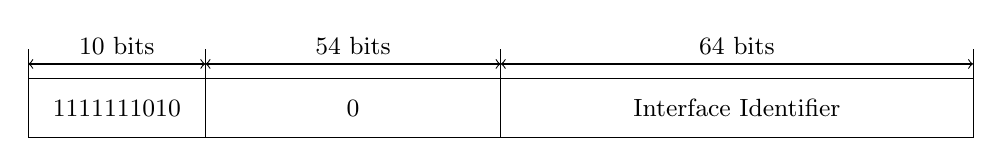
\begin{tikzpicture}[scale=0.75]
		\draw (0,0) rectangle (16,1);
		\draw (0,1) -- ++(0,0.5);
		\draw (3,0) -- ++(0,1.5);
		\draw (8,0) -- ++(0,1.5);
		\draw (16,1) -- ++(0,0.5);
		\node at (1.5, 0.5) {\small 1111111010};
		\node at (5.5, 0.5) {\small 0};
		\node at (12, 0.5) {\small Interface Identifier};
		\draw[<->] (0,1.25) -- (3,1.25) node[midway, above] {\small 10 bits};
		\draw[<->] (3,1.25) -- (8,1.25) node[midway, above] {\small 54 bits};
		\draw[<->] (8,1.25) -- (16,1.25) node[midway, above] {\small 64 bits};
	\end{tikzpicture}
	\end{center}
	\caption{Link Local Unicast address}
	\label{fig:ipv6_ll_unicast}
\end{figure}

An interface can have several addresses, but must at least have one Link-Local Unicast address.
The Link-Local Unicast address is formed as shown in \autoref{fig:ipv6_ll_unicast}.

\begin{figure}[htp]
	\begin{center}
	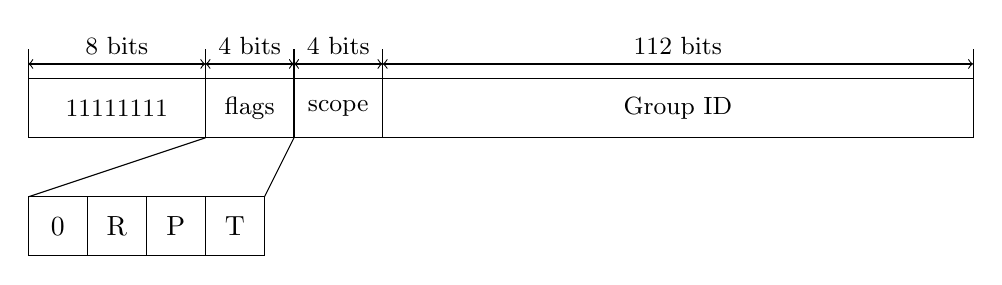
\begin{tikzpicture}[scale=0.75]
		\draw (0,2) rectangle (16,3);
		\draw (0,3) -- ++(0,0.5);
		\draw (3,2) -- ++(0,1.5);
		\draw (4.5,2) -- ++(0,1.5);
		\draw (6,2) -- ++(0,1.5);
		\draw (16,3) -- ++(0,0.5);
		\node at (1.5, 2.5) {\small 11111111};
		\node at (3.75, 2.5) {\small flags};
		\node at (5.25, 2.5) {\small scope};
		\node at (11, 2.5) {\small Group ID};
		\draw[<->] (0,3.25) -- ++(3,0) node[midway, above] {\small 8 bits};
		\draw[<->] (3,3.25) -- ++(1.5,0) node[midway, above] {\small 4 bits};
		\draw[<->] (4.5,3.25) -- ++(1.5,0) node[midway, above] {\small 4 bits};
		\draw[<->] (6,3.25) -- (16,3.25) node[midway, above] {\small 112 bits};

		\draw (3,2) -- (0,1);
		\draw (4.5,2) -- (4,1);
		\draw (0,0) rectangle (4,1);
		\node at (0.5,0.50) {0};
		\draw (1,0) -- ++(0,1);
		\node at (1.5,0.50) {R};
		\draw (2,0) -- ++(0,1);
		\node at (2.5,0.50) {P};
		\draw (3,0) -- ++(0,1);
		\node at (3.5,0.50) {T};
	\end{tikzpicture}
	\end{center}
	\caption{Multicast address}
	\label{fig:ipv6_multicast_addr}
\end{figure}

\begin{table}
	\centering
	\caption{Multicast Scopes}
	\begin{tabular}{|c|l|} \hline
	Number & Scope              \\ \hline \hline
	0      & reserved           \\ \hline
	1      & Interface-Local    \\ \hline
	2      & Link-Local         \\ \hline
	3      & reserved           \\ \hline
	4      & Admin-Local        \\ \hline
	5      & Site-Local         \\ \hline
	6-7    & unassigned         \\ \hline
	8      & Organization-Local \\ \hline
	9-D    & unassigned         \\ \hline
	E      & Global             \\ \hline
	F      & reserved           \\ \hline
	\end{tabular}
	\label{tab:mcast_scopes}
\end{table}

The multicast address format depicted in \autoref{fig:ipv6_multicast_addr}.
The highest byte is the multicast prefix 0xff, followed by four bits flags, and four bits scope.
For the flags, only the T flag is of interest in this work.
The T-flag signals an unassigned address when it's set to one.
If the T-flag is zero, the address is a "well-known" address.
The scopes are listed in \autoref{tab:mcast_scopes}.

\newpage

Some predefined multicast addresses are, for example:
\begin{itemize}
	\item ff01::1 Interface-Local All-Nodes multicast address
	\item ff02::1 Link-Local All-Nodes multicast address
	\item ff02::2 Link-Local All-Routers multicast address
	\item ff02::2 Site-Local All-Routers multicast address
	\item ff02:0:0:0:0:1:ffXX:XXXX Solicited-Node multicast address
\end{itemize}
The Solicited-Node multicast address is formed by the prefix ff02:0:0:0:0:1:ff::/104 concatenated with the low-order 24 bits of the unicast or anycast address.

\begin{figure}[htp]
	\begin{center}
	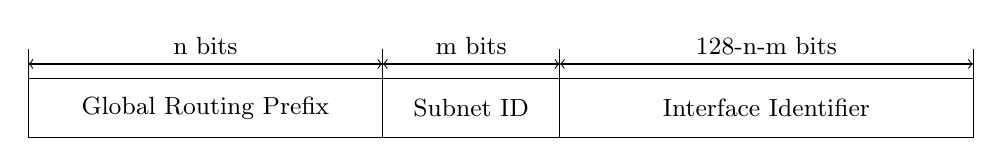
\begin{tikzpicture}[scale=0.75]
		\draw (0,0) rectangle (16,1);
		\draw (0,1) -- ++(0,0.5);
		\draw (6,0) -- ++(0,1.5);
		\draw (9,0) -- ++(0,1.5);
		\draw (16,1) -- ++(0,0.5);
		\node at (3, 0.5) {\small Global Routing Prefix};
		\node at (7.5, 0.5) {\small Subnet ID};
		\node at (12.5, 0.5) {\small Interface Identifier};
		\draw[<->] (0,1.25) -- (6,1.25) node[midway, above] {\small n bits};
		\draw[<->] (6,1.25) -- (9,1.25) node[midway, above] {\small m bits};
		\draw[<->] (9,1.25) -- (16,1.25) node[midway, above] {\small 128-n-m bits};
	\end{tikzpicture}
	\end{center}
	\caption{Global Unicast address}
	\label{fig:ipv6_global_unicast}
\end{figure}

A Global Unicast Address, as shown in \autoref{fig:ipv6_global_unicast} consists of a global routing prefix, a subnet ID, and the IID.
Global unicast addresses not starting with binary 000 always have an IID length of 64 bytes, same as the Link-Local Unicast address.
The global routing prefix is a value assigned to a site and distributed by the routers on that site.
The Subnet ID is an identifier of a link within the site.
The global unicast address is used to address single nodes that are not Link-Local, for example, a node on the internet.

A node must at least listen to the following addresses:
\begin{itemize}
	\item The Link-Local addresses assigned to the interfaces
	\item The loopback address
	\item The All-Nodes multicast address
	\item The Solicited-Nodes multicast address for each anycast and multicast address
	\item All multicast addresses for multicast groups the node has joined
\end{itemize}

\subsection{IPv6 Header}
\label{sec:ipv6_hdr}
\begin{figure}[htp]
	\begin{center}
	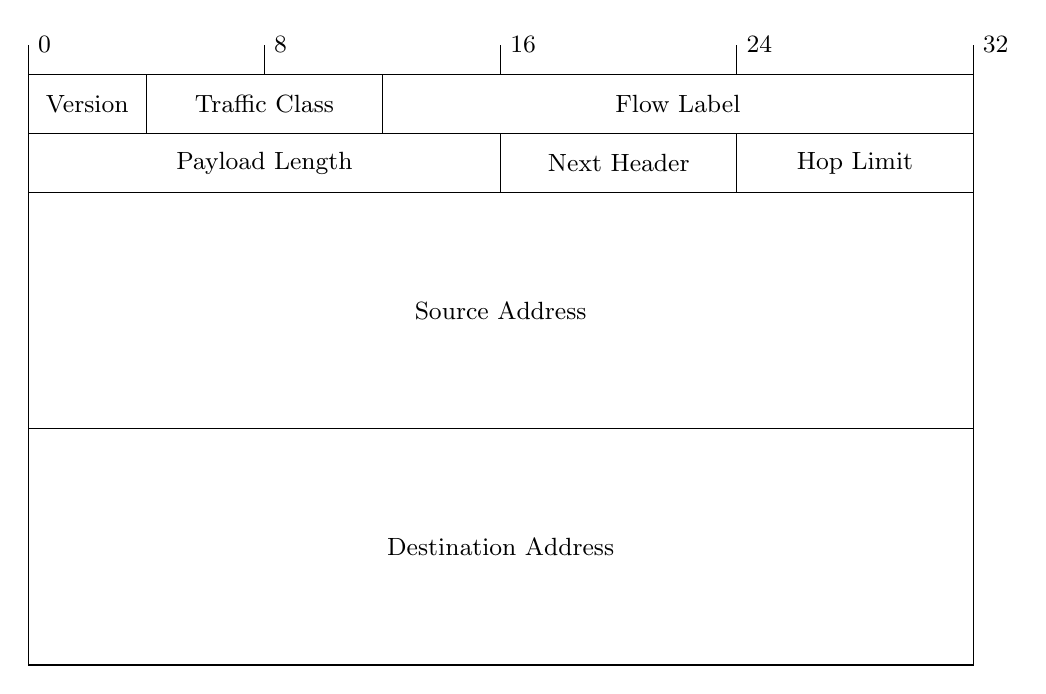
\begin{tikzpicture}[scale=0.75]
		\draw (0,0) -- (16,0) -- (16,10) -- (0,10) -- cycle;
		\draw (0,9) -- (16,9);
		\draw (0,8) -- (16,8);
		\draw (0,4) -- (16,4);
		\draw (0,10) -- ++(0,0.5) node[right] {\small 0};
		\draw (4,10) -- ++(0,0.5) node[right] {\small 8};
		\draw (8,10) -- ++(0,0.5) node[right] {\small 16};
		\draw (12,10) -- ++(0,0.5) node[right] {\small 24};
		\draw (16,10) -- ++(0,0.5) node[right] {\small 32};

		\draw (2,10) -- (2,9);
		\node at (1,9.5) {\small Version};
		\draw (6,10) -- (6,9);
		\node at (4, 9.5) {\small Traffic Class};
		\node at (11, 9.5) {\small Flow Label};

		\draw (8,9) -- (8,8);
		\node at (4, 8.5) {\small Payload Length};
		\draw (12,9) -- (12,8);
		\node at (10, 8.5) {\small Next Header};
		\node at (14,8.5) {\small Hop Limit};

		\node at (8, 6) {\small Source Address};
		\node at (8, 2) {\small Destination Address};
	\end{tikzpicture}
	\end{center}
	\caption{IPv6 Header}
	\label{fig:ipv6_hdr}
\end{figure}

The IPv6 header, as shown in \autoref{fig:ipv6_hdr}, has a fixed size of 40 bytes.
The fixed length makes it easier to process IPv6 headers and allows simple compression schemes like IPHC \cite{rfc6282}.

The 4-bit Version field is always 0x6 for IPv6.
Traffic-Class has a length of eight bits where the six most significant bits correspond to the Differentiated Service (DS) \cite{rfc2474} and
the remaining two bits are used for Explicit Congestion Notification (ECN) \cite{rfc3168}.
The 16-bit Payload Length field is an unsigned integer, defining the remaining length of the packet.
This number excludes the IP header but includes all possible next headers.
The next header field identifies the header type of the following extension- or protocol-header, if any, or "No Next Header" (59) if there aren't any.

The concept of Next Headers instead of options makes IPv6 very flexible.
Any number of options headers may follow the IPv6 header in a chained manner.
Therefor, every option header includes another next header field, forming a chain until the next header is an upper-layer protocol or the "No Next Header" option.

The Hop Limit is a counter, initialized by the node that issued the packet, with the desired limit of how many times this packet may be forwarded.
Every hop that forwards, a router, for example, decrements the hop limit by one.
When the limit reaches zero, the packet is discarded, and the node sends a message back to the source to inform about the discarding.

The Source Address is the IP address of the interface, and the Destination Address is the IP address of the desired receiver.
The Source Address and Destination Address both have a length of 128 bits.

IPv6 supports fragmentation, where a packet is cut into smaller fragments at the sender, transported, and reassembled at the destination.
For fragmentation, the Fragment Header is used.
Packet fragmentation is only allowed at the sender. Routers are not allowed to fragment packets.
IPv6 requires a minimal Maximum Transfer Unit (MTU) of 1280 bytes, which is the minimum link MTU that must be supported by every node on the internet.
Links that are not capable of transferring packets of at last 1280 bytes must apply fragmentation and reassembly at the Data-Link Layer.

\subsection{ICMPv6}
\label{sec:icmp_v6}

\begin{figure}[htp]
	\begin{center}
	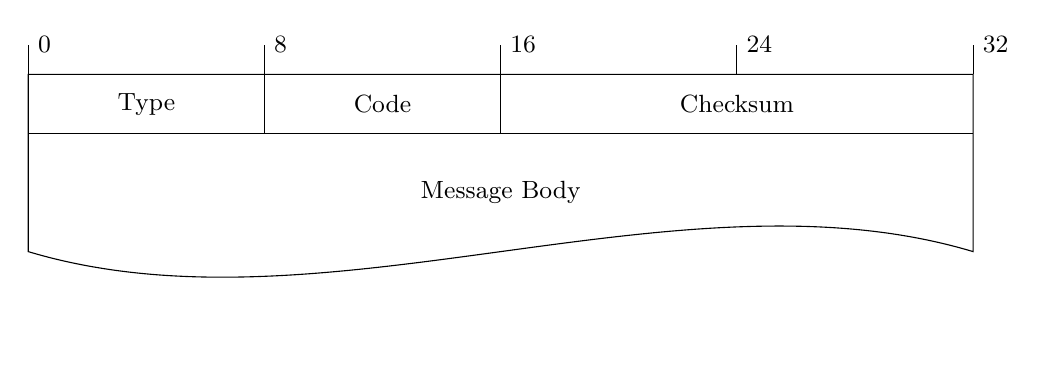
\begin{tikzpicture}[scale=0.75]
		\draw (0,0) .. controls (5, -1.5) and (11,1.5) .. (16,0) -- (16,3) -- (0,3) -- cycle;
		\draw (0,3) -- ++(0,0.5) node[right] {\small 0};
		\draw (4,3) -- ++(0,0.5) node[right] {\small 8};
		\draw (8,3) -- ++(0,0.5) node[right] {\small 16};
		\draw (12,3) -- ++(0,0.5) node[right] {\small 24};
		\draw (16,3) -- ++(0,0.5) node[right] {\small 32};

		\draw (4,2) -- ++(0,1);
		\node at (2,2.5) {\small Type};
		\draw (8,2) -- ++(0,1);
		\node at (6, 2.5) {\small Code};
		\node at (12, 2.5) {\small Checksum};
		\draw (0,2) -- ++(16,0);

		\node at (8,1) {\small Message Body};
	\end{tikzpicture}
	\end{center}
	\caption{Internet Control Message Protocol Format}
	\label{fig:icmp_format}
\end{figure}

\begin{table}
	\centering
	\caption{ICMPv6 Types defined by RFC4443}
	\begin{tabular}{|c|l|l|} \hline
	Type & Name                    & Description \\ \hline \hline
	1    & Destination Unreachable & \makecell[l]{Packet cannot be delivered to \\ its destination}                                  \\ \hline
	2    & Packet Too Big          & \makecell[l]{Router cannot forward the packet \\ because it exceeds a link-MTU}                 \\ \hline
	3    & Time Exceeded           & \makecell[l]{Router received a packet with a \\ hop-limit of zero or decremented \\ it to zero} \\ \hline
	4    & Parameter Problem       & \makecell[l]{Node detected a problem on a header \\ field that cannot be resolved}              \\ \hline
	128  & Echo Request            & A request to reply back to the sender                                                           \\ \hline
	129  & Echo Reply              & The reply to the Echo request                                                                   \\ \hline
	\end{tabular}
	\label{tab:ipv6_icmp_types}
\end{table}

ICMPv6 is a Transport-Layer protocol defined in \cite{rfc4443}.
\autoref{fig:icmp_format} depicts the ICMPv6 header format.
\autoref{tab:ipv6_icmp_types} shows ICMPv6 Types defined directly by the ICMPv6 RFC.
Other types are defined in the respective RFCs defining ICMPv6 messages.

\subsection{Neighbor Discovery Protocol}
\label{sec:ipv6_ndp}

\begin{figure}[htp]
	\begin{tikzpicture}[
		psuite/.style={
			draw=black,
			rounded corners,
			rectangle, 
			minimum width=3.5cm,
			minimum height=0.75cm,
			font=\small},
		frame/.style= {
			draw=black,
			rectangle, 
			minimum width=1.75cm,
			minimum height=0.5cm,
			font=\tiny}]
		\node (app) [psuite, fill=orange!30] {Application};
		\node [right of=app, xshift=9.25cm, frame, fill=orange!30] {App data};
		\node (transp) [below of=app, psuite, fill=green!30] {Transport};
		\node [right of=transp, xshift=9.25cm, frame, fill=orange!30] {App data};
		\node [right of=transp, xshift=7.5cm, frame, fill=green!30] {Next Header};
		\node (inet) [below of=transp, psuite, fill=blue!30] {Internet};
		\node [right of=inet, xshift=9.25cm, frame, fill=orange!30] {App data};
		\node [right of=inet, xshift=7.5cm, frame, fill=green!30] {Next Header};
		\node [right of=inet, xshift=5.75cm, frame, fill=blue!30] {IPv6 Header};
		\node (link) [below of= inet, psuite, fill=red!30] {Link};
		\node [right of=link, xshift=9.25cm, frame, fill=orange!30] {App data};
		\node [right of=link, xshift=7.5cm, frame, fill=green!30] {Next Header};
		\node [right of=link, xshift=5.75cm, frame, fill=blue!30] {IPv6 Header};
		\node [right of=link, xshift=4cm, frame, fill=red!30] {Link Header};

		\draw [thick, ->]($(app.east) + (0.8cm,0)$) -- ($(link.east) + (0.8cm,0)$) node[midway, above = 0.1, rotate=90] {\small Send};
		\draw [thick, <-]($(app.east) + (1.2cm,0)$) -- ($(link.east) + (1.2cm,0)$) node[midway, above = 0.1, rotate=270] {\small Receive};

		\node [above of=app, yshift=0.25cm] {Internet Protocol Suite};
		\node [above of=app, yshift=0.25cm, xshift=8cm] {Frame};

		\begin{scope}[on background layer]
			\fill [black!15] ($(app.north west) + (-0.25cm, 0.25)$) rectangle ($(link.south east)+ (0.25cm, -0.25)$);
			\fill [black!15] ($(app.north) + (3.75cm, 0.25)$) rectangle ($(link.south)+ (11.5cm, -0.25)$);
		\end{scope}

	\end{tikzpicture}
	\caption{IPv6 Header Encapsulation}
	\label{fig:ipv6_encapsulation}
\end{figure}


\autoref{fig:ipv6_encapsulation} shows how the data and headers of the upper layers get encapsulated in an IPv6 datagram that gets finally encapsulated in a frame.
IPv6 works on 128-bit addresses, but nodes use different addresses on their Link-Layer to transmit the frames.
This so-called Link-Layer address could either be the address of the receiver directly on the link or the Link-Layer address of the router
in case the receiver is not in the same Link-Local network.
The Link-Layer address of the next hop or the destination, in case of a Link-Local transfer, needs to be discovered first.
IPv6 uses the Link-Layer Neighbor Discovery protocol (NDP) \cite{rfc4861} for this task.
NDP packets are encapsulated in ICMPv6 (Internet Control Message Protocol) messages.
The nodes use a so-called Neighbor Cache to learn the relevant addresses of its neighborhood.
Addresses that have been resolved once stay in the cache for a predefined time.
For this time, the address does not need to be resolved but can be taken from the cache.

\begin{figure}[htp]
	\begin{center}
	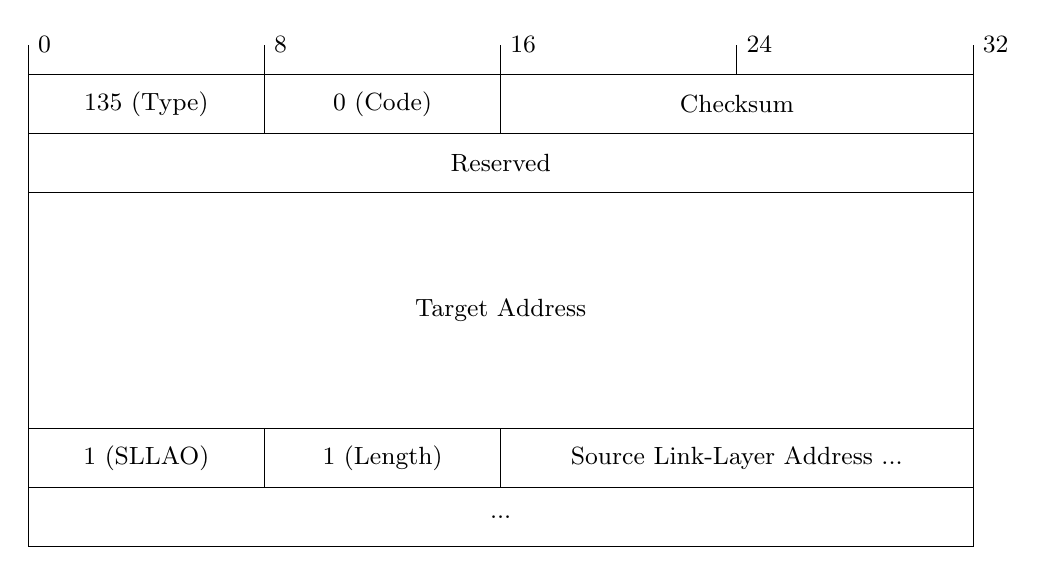
\begin{tikzpicture}[scale=0.75]
		\draw (0,0) -- (16,0) -- (16,8) -- (0,8) -- cycle;
		\draw (0,8) -- ++(0,0.5) node[right] {\small 0};
		\draw (4,8) -- ++(0,0.5) node[right] {\small 8};
		\draw (8,8) -- ++(0,0.5) node[right] {\small 16};
		\draw (12,8) -- ++(0,0.5) node[right] {\small 24};
		\draw (16,8) -- ++(0,0.5) node[right] {\small 32};

		\draw (4,8) -- (4,7);
		\node at (2,7.5) {\small 135 (Type)};
		\draw (8,8) -- (8,7);
		\node at (6, 7.5) {\small 0 (Code)};
		\node at (12, 7.5) {\small Checksum};
		\draw (0,7) -- ++(16,0);

		\node at (8, 6.5) {\small Reserved};
		\draw (0,6) -- ++(16,0);

		\node at (8, 4) {\small Target Address};
		\draw (0,2) -- ++(16,0);
		
		\draw (4,2) -- (4,1);
		\node at (2,1.5) {\small 1 (SLLAO)};
		\draw (8,2) -- (8,1);
		\node at (6, 1.5) {\small 1 (Length)};
		\node at (12, 1.5) {\small Source Link-Layer Address ...};
		\draw (0,1) -- ++(16,0);
		\node at (8, 0.5) {\small ...};

	\end{tikzpicture}
	\end{center}
	\caption{Neighbor Solicitation Message Example}
	\label{fig:ipv6_ns}
\end{figure}
\input{figures/ipv6_ndp_na}

NDP defines two message formats for finding direct neighbors.
\begin{itemize}
	\item Neighbor Solicitation Message Format
	\item Neighbor Advertisement Message Format
\end{itemize}

\newpage

Neighbor Advertisement messages propagate a node's Link-Layer address to other nodes.
They are broadcasted when the node joins a network or can be requested by a Neighbor Solicitation message (NS).
NAs not requested by an NS are called unsolicited advertisements and typically sent to the all-node multicast address.
The node can send an NA message to the solicited-node multicast address and wait for an NA from the targeted node to resolve an address.
The node can send an NS message to the targeted nodes unicast address to check if the node is still available.

\autoref{fig:ipv6_ns} shows an example of a Neighbor Solicitation message.
The ICMPv6 Type of an NS is 135, and the code is always zero for an NS message.
The Target Address field contains the IPv6 address of the node, where the NA should be requested.
The Target Address is followed by the option field.
In case the source of the IP header is not the unspecified address (::), the option field must include the Source Link-Layer Address option (SLLAO).
The length field of a Link-Layer Address Option (LLAO) describes the total length of the option field in eight-bytes units.
For example, if the Link-Layer address has a length of six bytes or smaller, the length field is one.

The answer to an NS message is the Neighbor Advertisement message (NA).
\autoref{fig:ipv6_na} depicts an example of such an NA message.
The ICMPv6 type field is always 136, and the code is always zero for an NA message.
The R-bit implies that the node, sending the NA, is a router.
A set S-bit means that the NA message is sent as a response to an NS message.
The O-bit indicates that this NA message should override a possibly cached Link-Layer address from a previously sent NA.
The Target Address can either be the address of the solicitation node or the all-nodes multicast address in case of an unsolicited NA or an unspecified source address.

\begin{figure}[htp]
	\begin{center}
	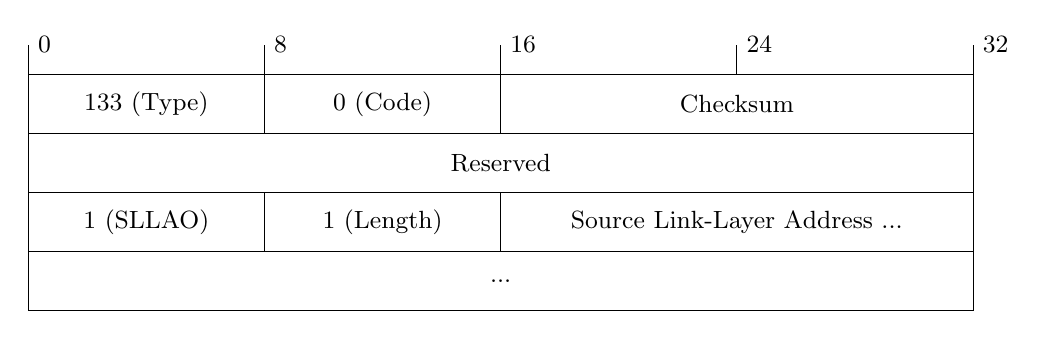
\begin{tikzpicture}[scale=0.75]
		\draw (0,0) rectangle (16,4);
		\draw (0,4) -- ++(0,0.5) node[right] {\small 0};
		\draw (4,4) -- ++(0,0.5) node[right] {\small 8};
		\draw (8,4) -- ++(0,0.5) node[right] {\small 16};
		\draw (12,4) -- ++(0,0.5) node[right] {\small 24};
		\draw (16,4) -- ++(0,0.5) node[right] {\small 32};

		\draw (4,4) -- (4,3);
		\node at (2,3.5) {\small 133 (Type)};
		\draw (8,4) -- (8,3);
		\node at (6, 3.5) {\small 0 (Code)};
		\node at (12, 3.5) {\small Checksum};
		\draw (0,3) -- ++(16,0);

		\node at (8, 2.5) {\small Reserved};
		\draw (0,2) -- ++(16,0);

		\draw (4,2) -- (4,1);
		\node at (2,1.5) {\small 1 (SLLAO)};
		\draw (8,2) -- (8,1);
		\node at (6, 1.5) {\small 1 (Length)};
		\node at (12, 1.5) {\small Source Link-Layer Address ...};
		\draw (0,1) -- ++(16,0);
		\node at (8, 0.5) {\small ...};

	\end{tikzpicture}
	\end{center}
	\caption{Router Solicitation Message Example}
	\label{fig:ipv6_rs}
\end{figure}
\begin{figure}[htp]
	\begin{center}
	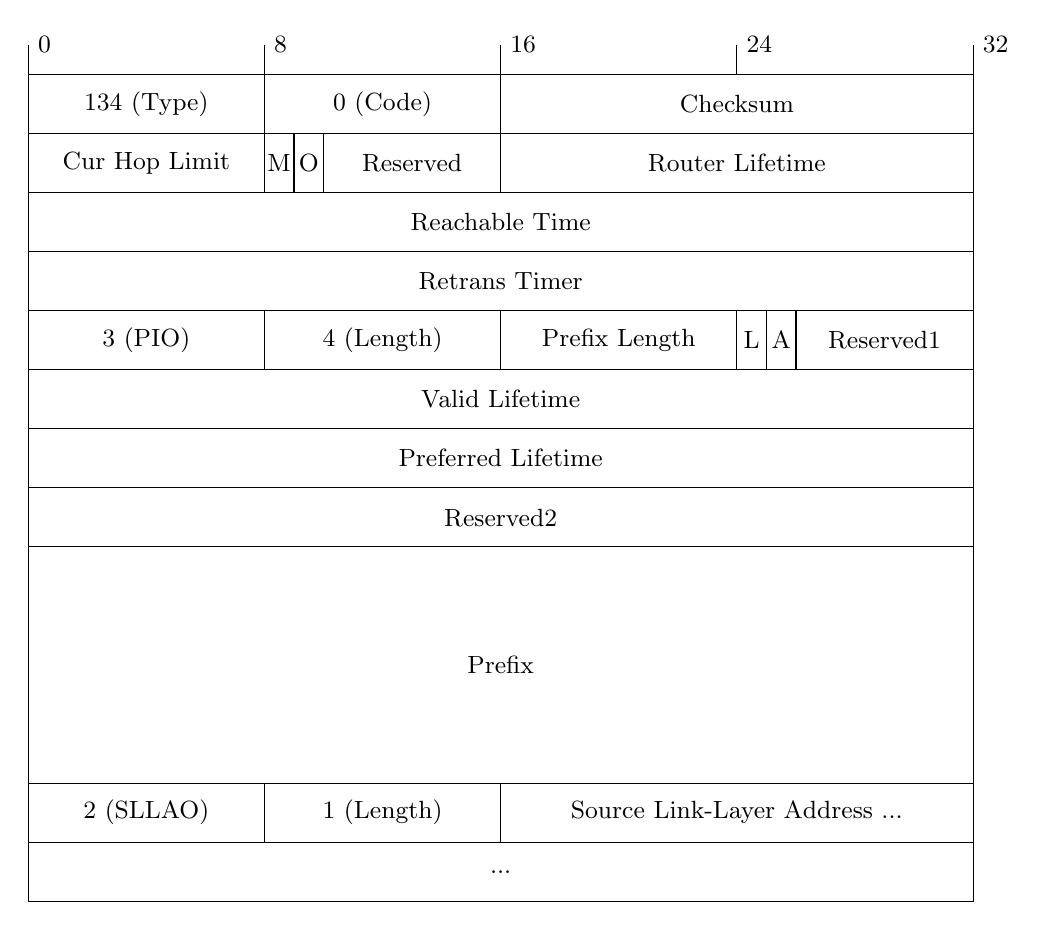
\begin{tikzpicture}[scale=0.75]
		\draw (0,0) rectangle (16,14);
		\draw (0,14) -- ++(0,0.5) node[right] {\small 0};
		\draw (4,14) -- ++(0,0.5) node[right] {\small 8};
		\draw (8,14) -- ++(0,0.5) node[right] {\small 16};
		\draw (12,14) -- ++(0,0.5) node[right] {\small 24};
		\draw (16,14) -- ++(0,0.5) node[right] {\small 32};
0
		\draw (4,13) -- ++(0,1);
		\node at (2,13.5) {\small 134 (Type)};
		\draw (8,13) -- ++(0,1);
		\node at (6, 13.5) {\small 0 (Code)};
		\node at (12, 13.5) {\small Checksum};
		\draw (0,13) -- ++(16,0);

		\draw (4,12) -- ++(0,1);
		\node at (2, 12.5) {\small Cur Hop Limit};
		\draw (4.5,12) -- ++(0,1);
		\node at (4.25, 12.5) {\small M};
		\draw (5,12) -- ++(0,1);
		\node at (4.75, 12.5) {\small O};
		\draw (8,12) -- ++(0,1);
		\node at (6.5, 12.5) {\small Reserved};
		\node at (12, 12.5) {\small Router Lifetime};
		\draw (0,12) -- ++(16,0);

		\node at (8, 11.5) {\small Reachable Time};
		\draw (0,11) -- ++(16,0);

		\node at (8, 10.5) {\small Retrans Timer};
		\draw (0,10) -- ++(16,0);

		\draw (4,9) -- ++(0,1);
		\node at (2,9.5) {\small 3 (PIO)};
		\draw (8,9) -- ++(0,1);
		\node at (6, 9.5) {\small 4 (Length)};
		\draw (12,9) -- ++(0,1);
		\node at (10, 9.5) {\small Prefix Length};
		\draw (12.5,9) -- ++(0,1);
		\node at (12.25, 9.5) {\small L};
		\draw (13,9) -- ++(0,1);
		\node at (12.75, 9.5) {\small A};
		\node at (14.5, 9.5) {\small Reserved1};
		\draw (0,9) -- ++(16,0);

		\node at (8,8.5) {\small Valid Lifetime};
		\draw (0,8) -- ++(16,0);
		\node at (8,7.5) {\small Preferred Lifetime};
		\draw (0,7) -- ++(16,0);
		\node at (8,6.5) {\small Reserved2};
		\draw (0,6) -- ++(16,0);
		\node at (8,4) {\small Prefix};
		\draw (0,2) -- ++(16,0);

		\draw (4,2) -- (4,1);
		\node at (2,1.5) {\small 2 (SLLAO)};
		\draw (8,2) -- (8,1);
		\node at (6, 1.5) {\small 1 (Length)};
		\node at (12, 1.5) {\small Source Link-Layer Address ...};
		\draw (0,1) -- ++(16,0);
		\node at (8, 0.5) {\small ...};

	\end{tikzpicture}
	\end{center}
	\caption{Router Advertisement Message Example}
	\label{fig:ipv6_ra}
\end{figure}

NDP defines two message formats for finding routers on the link.
\begin{itemize}
	\item Router Solicitation Message Format
	\item Router Advertisement Message Format
\end{itemize}

Router advertisement messages (RA) propagate information about routers on the link.
Unsolicited router advertisements are sent out to the all-nodes multicast address by the routers periodically.
A node can also request a router advertisement by sending out a Router Solicitation (RS) message to the all-routers multicast group.
The router will then answer with an RA to the issuer's unicast address.
The RS message is shown in \autoref{fig:ipv6_rs}.

The RA message is shown in \autoref{fig:ipv6_ra}.
The ICMPv6 Type of an RA is 134, and the code is always zero for an RA message.
The Current Hop Limit field tells the receiving node which hop-limit should be used for outgoing packets.
Zero means unspecified. The M and O flags are DHCPv6 related and not relevant for this work.
The Router Lifetime field is an unsigned 16-bit value in units of a second. It specifies the lifetime associated with the default router.
The Reachable Time specifies a time interval in milliseconds for which a node can assume that an already discovered node is still reachable.
The last timer field, the Retrans Timer, defines the time between the retransmission of a Neighbor Solicitation message in units of milliseconds.
The RA example has two option fields included. The Prefix Info and the SLLAO.
The SLLAO includes the source Link-Layer address like the RS message.
The Prefix Info option (PIO) tells the receiving node information about the prefix used for address autoconfiguration.
The length value indicates the number of bits used as the prefix. The prefix is always in the upper address bytes since the address
in this option has the same length ass an entire address.
The L-Flag indicates that the prefix is on-link, which means that it can be reached directly without any router involved.
The A-Flag signals the prefix can be used for Stateless Address Autoconfiguration.
Valid Lifetime and Preferred Lifetime signal the SLAAC for how long the address is valid and for how long it should be used.
All-ones (0xffffffff) values signal infinite lifetime.

\subsection{Stateless Address Autoconfiguration}
\label{sec:ipv6_slaac}

\begin{figure}[htp]
	\begin{center}
	\begin{tikzpicture}[scale=0.45, node distance=2cm, every node/.append style={scale=0.45}]
		\node (start) [startstop] {Interface up};
		\node (ll_ten) [process, below = of start] {Create tentative Link-Local address};
		\node (dad_ns) [io, below = of ll_ten] {Send NS message with tentative Link-Local address (DAD)};
		\node (dad_na) [io, below = of dad_ns] {Wait for NA message with tentative Link-Local address (DAD) or Timeout};
		\node (dad) [decision, below = of dad_na] {NA message received?};
		\node (alt_addr) [decision, right of=dad, xshift=7cm] {Alternative address?};
		\node (dad_fail) [startstop, below = of alt_addr] {DAD failed};
		\node (ll) [process, below = of dad] {Apply Link-Local address};
		\node (rs) [io, below = of ll] {Send RS};
		\node (ra) [io, below = of rs] {Wait for RA};
		\node (glob_create) [process, below = of ra] {Create tentative global address};
		\node (dad_ns_glob) [io, below = of glob_create] {Send NS message with global address from RA prefix (DAD)};
		\node (dad_na_glob) [io, below = of dad_ns_glob] {Wait for NA message with global address from RA prefix (DAD) or Timeout};
		\node (dad_glob) [decision, below = of dad_na_glob] {NA message received?};
		\node (glob) [process, below = of dad_glob] {Apply global address};

		\draw [arrow] (start) -- (ll_ten);
		\draw [arrow] (ll_ten) -- (dad_ns);
		\draw [arrow] (dad_ns) -- (dad_na);
		\draw [arrow] (dad_na) -- (dad);
		\draw [arrow] (dad) -- node [anchor=south] {yes (DAD failed)} (alt_addr);
		\draw [arrow] (dad) -- node [anchor=east] {no (DAD succeeded)} (ll);
		\draw [arrow] (alt_addr) |- node [anchor=south] {yes} (ll_ten);
		\draw [arrow] (alt_addr) -- node [anchor=east] {no} (dad_fail);
		\draw [arrow] (ll) -- (rs);
		\draw [arrow] (rs) -- (ra);
		\draw [arrow] (ra) -- (glob_create);
		\draw [arrow] (glob_create) -- (dad_ns_glob);
		\draw [arrow] (dad_ns_glob) -- (dad_na_glob);
		\draw [arrow] (dad_na_glob) -- (dad_glob);
		\draw [arrow] (dad_glob) -- node [anchor=east] {no (DAD succeeded)} (glob);
		\coordinate [right = of ra] (ra_right) ;
		\draw [arrow] (dad_glob.east) -- ++(2cm,0) node [anchor=south] {yes (DAD failed)} -|   (ra_right) -- (ra.east);
		\draw [arrow] (glob.south) -- ++(0,-1cm) -| (ra_right) -- (ra);
	\end{tikzpicture}
	\end{center}
	\caption{Stateless Address Autoconfiguration}
	\label{fig:ipv6_slaac}
\end{figure}

IPv6 nodes use the Stateless Address Autoconfiguration (SLAAC), defined in RFC4862 \cite{rfc4862}, to configure  the interface's addresses.
The SLAAC mechanism generates Link-Local and global addresses.
The Link-Local address is formed by combining the Link-Local prefix with the IID, and global addresses use the prefix
learned from RA messages, combined with the IID.
\autoref{fig:ipv6_slaac} shows the routine to perform SLAAC.
When an interface is initialized, it assigns itself a tentative Link-Local address, formed as described above.
Then the node sends out an NS message with the Target Address of the tentatively chosen address.
The source IPv6 address is the unspecified address (::) and the destination IPv6 address is the solicited multicast address.
This process is called Duplicate Address Detection (DAD).
If there is a node on the link, using the same address, it returns an NA message, indicating a duplication, and the node then discards
the tentative address and depending on the configuration, generates a new address.
After the DAD, the node has a Link-Local address assigned and can send an RS.
All routers in the network answer the RS with an RA message where the node can get the prefix information from.
With this prefix information, the node forms a global address and starts listening to that address.

\FloatBarrier

\section{6lo}
\label{sec:6lo}

\begin{figure}[htp]
	\begin{tikzpicture}[
		layer/.style={
			minimum width=13cm,
			text width=13cm,
			minimum height=1.5cm,
			fill=black!5,
			align=left,
			node distance=0,
			font=\small},
		example/.style={
				draw=black,
				fill=white,	
				rectangle, 
				minimum width=2.5cm,
				minimum height=0.75cm,
				font=\small},
		node distance=0.25cm and 1cm]
\begin{scope}[on background layer]
		\node (app) [layer] {Application};
		\node (transp) [below = of app, layer] {Transport};
		\node (inet) [below = of transp, layer] {Internet};
		\node (link) [below = of inet, yshift=-0.5cm,layer] {Link};
		\node at (link) (adapt)  [fill=green!20, text width=9cm, minimum height=1cm, align=left, xshift=-2cm, yshift=0.85cm] {6lo Adaption};
\end{scope}
		\node (app_http) [right of = app, xshift=-2.5cm, example] {HTTP};
		\node (app_coap) [right = of app_http, example] {CoAP};
		\node (app_mqtt) [right = of app_coap, example] {MQTT};
		\node (transp_udp) [right of = transp, xshift=-2.5cm, example] {UDP};
		\node (transp_tcp) [right = of transp_udp, example] {TCP};
		\node (transp_icmp) [right = of transp_tcp, example] {ICMPv6};
		\node (inet_ipv6) [right of = inet, xshift=1cm, example, minimum width=9cm] {IPv6};
		\node (link_wpan) [right of = link, xshift=-2.5cm, example] {802.15.4};
		\node (link_can) [right = of link_wpan, example] {CAN};
		\node (adapt_6lowpan) [above = of  link_wpan, yshift=-0.2cm, example] {6LoWPAN};
		\node (adapt_6locan) [above = of link_can, yshift=-0.2cm, example] {6LoCAN};
		\node (link_eth) [right = of link_can, example] {Ethernet};
	\end{tikzpicture}
	\caption{6lo Adaption layer example}
	\label{fig:6lo_layer}
\end{figure}


6lo is the name of an Internet Engineering Task Force (IETF) Working Group (WG).
The 6lo WG focus on IPv6 connectivity over constrained nodes.
The nodes are constrained in the sense of limited power, memory, and lack of some required Link-Layer services.
The WG is working on IPv6-over-foo adaption layers, using specifications from 6LoWPAN technologies like RFC4944 \cite{rfc4944} and RFC6282 \cite{rfc6282}.
6lo technologies usually have a 6lo adaption-layer, as shown in \autoref{fig:6lo_layer}.

\subsection{IP Header Compression}
\label{sec:iphc}

For this document, the concept of the Adaption layer and the IP Header Compression (IPHC) is of importance.
The IPHC reduces redundant information in the 40 bytes IPv6 header.
The payload length, for example, is usually known from the Link-Layer packet size and is therefore always elided.
The version field is also always elided because the compression is only defined for IPv6.
Fields that can be recovered from Link-Layer information can be fully elided.
Fields filled with default parameters can either be entirely elided or chosen on a set of default values.
On a Link-Layer where the Interface Identifier (IID) is generated from the Link-Layer address,
the IPv6 header with a Link-Local source and Link-Local destination address, the IPv6 addresses in the header are
redundant and can be reconstructed from the Link-Layer headers.
This saves up to 38 bytes of data.
The compression can either be stateless or context-based.
A context is a global routing prefix that is known by all nodes and has an index.
This 4-bit index can then be used instead of transmitting the 64-bit prefix.
The distribution of the contexts is out of scope and not defined by aby standard yet.

\begin{figure}[htp]
	\begin{center}
	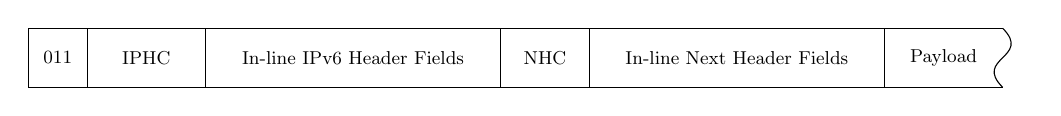
\begin{tikzpicture}[scale=0.75, every node/.append style={scale=0.75}]
		\draw (0,0) -- ++(16.5,0);
		\draw (0,1) -- ++(16.5,0);
		\draw (0,0) -- ++(0,1);
		\draw (16.5,0) .. controls (16,0.5) and (17,0.5) .. (16.5,1);

		\draw (1,0) -- ++(0,1);
		\node at (0.5, 0.5) {\small 011};

		\draw (3,0) -- ++(0,1);
		\node at (2, 0.5) {\small IPHC};

		\draw (8,0) -- ++(0,1);
		\node at (5.5, 0.5) {\small In-line IPv6 Header Fields};

		\draw (9.5,0) -- ++(0,1);
		\node at (8.75, 0.5) {\small NHC};

		\draw (14.5,0) -- ++(0,1);
		\node at (12, 0.5) {\small In-line Next Header Fields};

		\node at (15.5, 0.5) {\small Payload};
	\end{tikzpicture}
	\end{center}
	\caption{IPHC Frame Format}
	\label{fig:6lo_iphc_frame}
\end{figure}

The IPHC dispatch is a bit-field at the beginning of a packet, as shown in \autoref{fig:6lo_iphc_frame}.
The dispatch signals a IPHC compressed packet.
IPv6 header fields that cannot be fully elided are carried in-line after the IPHC bit-field.
The order of the in-lined data follows the order of the IPHC bit-field from left to right.
If the Next Header is compressible, the Next Header Compression (NHC) field follows the In-Line Header Fields.
Next-Header fields that cannot be fully elided, follow the NHC.

\begin{figure}[htp]
	\begin{center}
	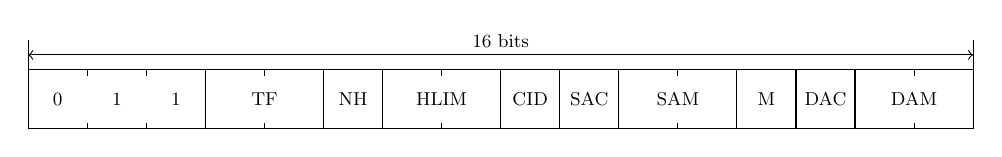
\begin{tikzpicture}[scale=0.75, every node/.append style={scale=0.75}]
		\draw (0,0) rectangle (16,1);
		\draw (0,1) -- ++(0,0.5);
		\draw (16,1) -- ++(0,0.5);
		\draw[<->] (0,1.25) -- (16,1.25) node[midway, above] {\small 16 bits};

		\foreach \x in {1,2,...,15}{
			\draw (\x,1) -- ++(0,-0.1);
			\draw (\x,0) -- ++(0,0.1);
		}

		\draw (3,0) -- ++(0,1);
		\node at (0.5, 0.5) {\small 0};
		\node at (1.5, 0.5) {\small 1};
		\node at (2.5, 0.5) {\small 1};

		\draw (5,0) -- ++(0,1);
		\node at (4, 0.5) {\small TF};

		\draw (6,0) -- ++(0,1);
		\node at (5.5, 0.5) {\small NH};

		\draw (8,0) -- ++(0,1);
		\node at (7, 0.5) {\small HLIM};

		\draw (9,0) -- ++(0,1);
		\node at (8.5, 0.5) {\small CID};

		\draw (10,0) -- ++(0,1);
		\node at (9.5, 0.5) {\small SAC};

		\draw (12,0) -- ++(0,1);
		\node at (11, 0.5) {\small SAM};

		\draw (13,0) -- ++(0,1);
		\node at (12.5, 0.5) {\small M};

		\draw (14,0) -- ++(0,1);
		\node at (13.5, 0.5) {\small DAC};

		\node at (15, 0.5) {\small DAM};

	\end{tikzpicture}
	\end{center}
	\caption{IPHC Format}
	\label{fig:6lo_iphc}
\end{figure}

The IPHC bit-field, including the three-bit dispatch (011), has a length of 16 bits, as shown in \autoref{fig:6lo_iphc}.

TF (Traffic-Class, Flow Label):\\
The first two bits define the Traffic-Class and Flow Label compression (TF).
The meaning of the values is stated in \autoref{tab:6lo_tf}.

\begin{table}[h!]
	\centering
	\caption{Traffic-Class and Flow-Label Compression}
	\begin{tabular}{|c|l|} \hline
	Code & Description                                           \\ \hline \hline
	00   & ECN + DSCP + 4-bit Pad + Flow Label (4 bytes)           \\ \hline
	01   & ECN + 2-bit Pad + Flow Label (3 bytes), DSCP is elided. \\ \hline
	10   & ECN + DSCP (1 byte), Flow Label is elided.              \\ \hline
	11   & Traffic-Class and Flow-Label are elided.                \\ \hline
	\end{tabular}
	\label{tab:6lo_tf}
\end{table}

NH (Next Header):\\
When this bit is set, the next header field is compressed, and the LOWPAN\_NHC (Next header compression) is following the in-line field.
Otherwise, the Next header byte is carried in-line.

HLIM (Hop Limit):\\
The HLIM field defines the compressed Hop Limit.

\begin{table}[h!]
	\centering
	\caption{Hop Limit Compression}
	\begin{tabular}{|c|l|} \hline
	Code & Description \\ \hline \hline
	00   & No compression. Carried in-line \\ \hline
	01   & The hop limit is 1              \\ \hline
	10   & The hop limit is 64             \\ \hline
	11   & The hop limit is 255            \\ \hline
	\end{tabular}
	\label{tab:6lo_hlim}
\end{table}

CID (Context Identifier Extension):\\
If set, an 8-bit Context Identifier is carried in-line. The format is shown in \autoref{fig:6lo_cid}.
If a context-based compression is used for source or destination-address, context zero is used.

\begin{figure}[htp]
	\begin{center}
	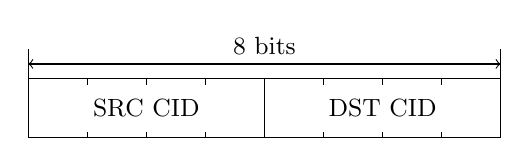
\begin{tikzpicture}[scale=0.75]
		\draw (0,0) rectangle (8,1);
		\draw (0,1) -- ++(0,0.5);
		\draw (8,1) -- ++(0,0.5);
		\draw[<->] (0,1.25) -- (8,1.25) node[midway, above] {\small 8 bits};

		\foreach \x in {1,2,...,7}{
			\draw (\x,1) -- ++(0,-0.1);
			\draw (\x,0) -- ++(0,0.1);
		}

		\draw (4,0) -- ++(0,1);
		\node at (2, 0.5) {\small SRC CID};
		\node at (6, 0.5) {\small DST CID};
	\end{tikzpicture}
	\end{center}
	\caption{Context ID Format}
	\label{fig:6lo_cid}
\end{figure}

SAC (Source Address Compression):\\
If set, the source address compression is context-based.
If not, it is stateless.

SAM (Source Address Mode):\\
The source address compression mode is interpreted differently for context-based or stateless compression.

The enumeration for stateless source address compression is shown in \autoref{tab:6lo_SAM_0}.
\begin{table}[h!]
	\centering
	\caption{Stateless Source and Destination-Address Compression}
	\begin{tabular}{|c|l|c|} \hline
	Code & Description                                           & In-lined bits\\ \hline \hline
	00   & No compression. Address is carried in-line            & 128 \\ \hline
	01   & \makecell[l]{The Prefix is fe80::/64.\\
	                    The IID is carried in-line}              & 64  \\ \hline
	10   & \makecell[l]{The Prefix is fe80::ff:fe00:XXXX/112.\\
	                    The last 16 bits are carried in-line}    & 16  \\ \hline
	11   & \makecell[l]{The Prefix is fe80::/64.\\
			    The IID is reconstructed from the\\
			    Link-Layer address.}                     & 0   \\ \hline
	\end{tabular}
	\label{tab:6lo_SAM_0}
\end{table}

The enumeration for context-based source address compression is shown in \autoref{tab:6lo_SAM_1}.
\begin{table}[h!]
	\centering
	\caption{Context-Based Source- and Destination-Address Compression}
	\begin{tabular}{|c|l|c|} \hline
	Code & Description                                                  & In-lined bits\\ \hline \hline
	00   & The unspecified address ::                                   & 0  \\ \hline
	01   & \makecell[l]{The Prefix is taken from the context. \\
	                    The IID is carried in-line.}                    & 64 \\ \hline
	10   & \makecell[l]{The Prefix is taken from the context. \\
			    Bits not covered by the context are \\
			    filled with ::ff:fe00:XXXX.\\
			    The last 16 bits are carried in-line}           & 16 \\ \hline
	11   & \makecell[l]{The Prefix is taken from the context.\\
			    The IID is reconstructed from the Link-Layer \\
			    address, if not covered by the context.}        & 0 \\ \hline
	\end{tabular}
	\label{tab:6lo_SAM_1}
\end{table}

M (Multicast Compression):\\
If set, the destination address is a multicast address.

DAC (Destination Address Compression):\\
If set, the destination address compression is context-based.
If not, it is stateless.

DAM (Destination Address Mode):\\
The interpretation of the destination address compression mode depends on the combination of multicast compression and destination address compression.

The enumeration for stateless non-multicast compression is shown in table \autoref{tab:6lo_SAM_0} and is the same as the compression for the source address.

The enumeration for context-based destination address compression is the same as the compression for the source address,
with the exception that case 00 is not allowed, and is shown in \autoref{tab:6lo_SAM_1}.

The enumeration for stateless multicast destination address compression is shown in 

\begin{table}[h!]
	\centering
	\caption{Stateless Multicast Destination-Address Compression}
	\begin{tabular}{|c|l|c|} \hline
	Code & Description                                   & In-lined bits\\ \hline \hline
	00   & No compression. Address is carried in-line    & 128 \\ \hline
	01   & The address takes the form ffXX::XX:XXXX:XXXX & 48  \\ \hline
	10   & The address takes the form ffXX::XX:XXXX      & 32  \\ \hline
	11   & The address takes the form ff02::XX           & 8   \\ \hline
	\multicolumn{3}{l}{Bytes marked as XX are carried in-line.}\\
	\end{tabular}
	\label{tab:6lo_DAC_M}
\end{table}

\begin{figure}[htp]
	\begin{center}
	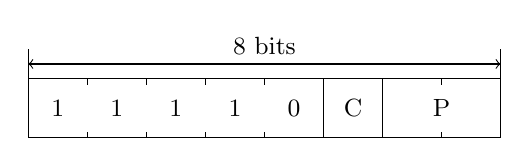
\begin{tikzpicture}[scale=0.75]
		\draw (0,0) rectangle (8,1);
		\draw (0,1) -- ++(0,0.5);
		\draw (8,1) -- ++(0,0.5);
		\draw[<->] (0,1.25) -- (8,1.25) node[midway, above] {\small 8 bits};

		\foreach \x in {1,2,...,7}{
			\draw (\x,1) -- ++(0,-0.1);
			\draw (\x,0) -- ++(0,0.1);
		}
		\foreach \x in {0.5,1.5,...,3.5}{
			\node at (\x, 0.5) {\small 1};
		}

		\node at (4.5, 0.5) {\small 0};
		\draw (5,0) -- ++(0,1);
		\node at (5.5, 0.5) {\small C};
		\draw (6,0) -- ++(0,1);
		\node at (7, 0.5) {\small P};
	\end{tikzpicture}
	\end{center}
	\caption{Next Header Compression for UDP Headers}
	\label{fig:6lo_nhc_udp}
\end{figure}

Another significant compression is the Next Header Compression, specifically the UDP header compression.
The format is shown in \autoref{fig:6lo_nhc_udp}. The first five bits are the dispatch for UDP header compression.

C (Checksum):
If C is set, the Checksum of the UDP datagram is elided or carried in-line otherwise.

P (Ports):
The enumeration of the port compression is shown in \autoref{tab:6lo_DAC}

\begin{table}[h!]
	\centering
	\caption{Stateless Multicast Destination Address Compression}
	\begin{tabular}{|c|l|c|} \hline
	Code & Description                                            & In-lined bits\\ \hline \hline
	00   & No compression. Both ports are carried in-line         & 32 \\ \hline
	01   & \makecell[l]{Source-Port fully in-lined.\\
	                    Destination port takes the form 0xf0XX}   & 24  \\ \hline
	10   & \makecell[l]{Destination Port fully in-lined.\\
	                    Source port takes the form 0xf0XX}        & 24  \\ \hline
	11   & Source- and Destination Port take the form 0xf0bX      & 8   \\ \hline
	\multicolumn{3}{l}{Bytes marked as XX are carried in-line.}\\
	\end{tabular}
	\label{tab:6lo_DAC}
\end{table}

\begin{figure}[htp]
	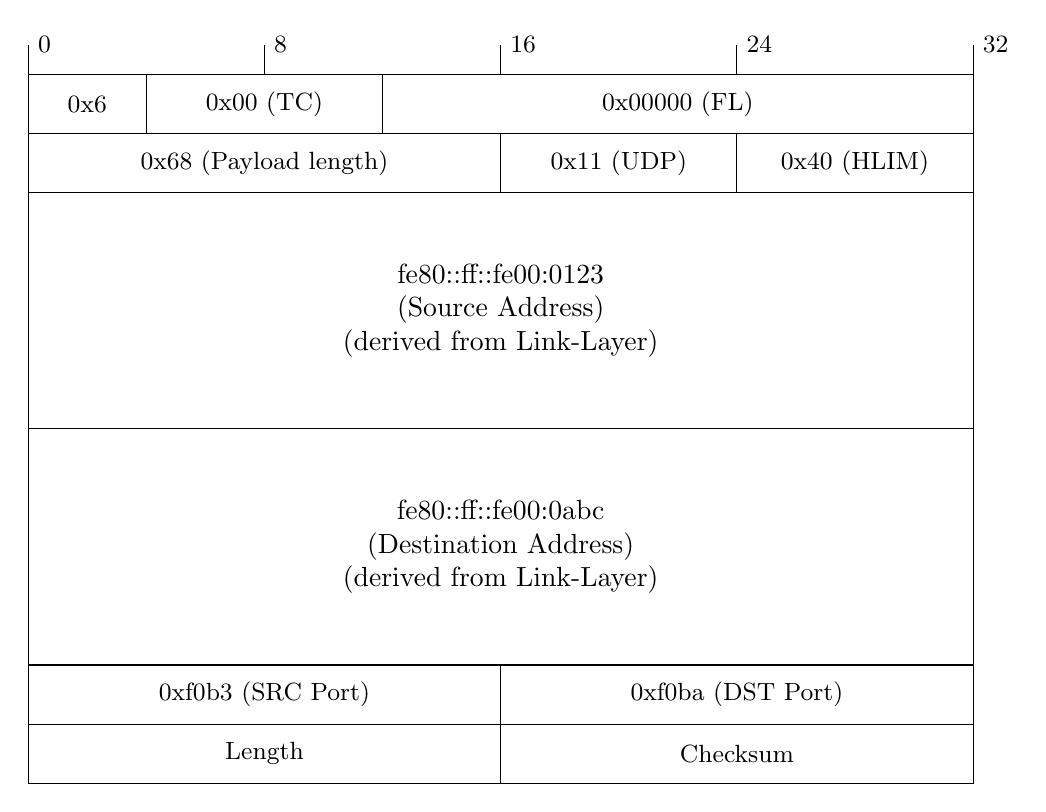
\begin{tikzpicture}[scale=0.75]
		%IPv6
		\draw (0,0) rectangle (16,12);
		\draw (0,11) -- (16,11);
		\draw (0,10) -- (16,10);
		\draw (0,6) -- (16,6);
		\draw (0,2) -- (16,2);
		\draw (0,1) -- (16,1);

		\draw (0,12) -- ++(0,0.5) node[right] {\small 0};
		\draw (4,12) -- ++(0,0.5) node[right] {\small 8};
		\draw (8,12) -- ++(0,0.5) node[right] {\small 16};
		\draw (12,12) -- ++(0,0.5) node[right] {\small 24};
		\draw (16,12) -- ++(0,0.5) node[right] {\small 32};

		\draw (2,12) -- ++(0,-1);
		\node at (1,11.5) {\small 0x6};
		\draw (6,12) -- ++(0,-1);
		\node at (4, 11.5) {\small 0x00 (TC)};
		\node at (11, 11.5) {\small 0x00000 (FL)};

		\draw (8,11) -- ++(0,-1);
		\node at (4, 10.5) {\small 0x68 (Payload length)};
		\draw (12,11) -- ++(0,-1);
		\node at (10, 10.5) {\small 0x11 (UDP)};
		\node at (14,10.5) {\small 0x40 (HLIM)};

		\node at (8, 8) [align=center] {fe80::ff::fe00:0123 \\(Source Address) \\ (derived from Link-Layer)};
		\node at (8, 4) [align=center] {fe80::ff::fe00:0abc \\ (Destination Address) \\ (derived from Link-Layer)};

		\draw (8,2) -- ++(0,-1);
		\node at (4,1.5) {\small 0xf0b3 (SRC Port)};
		\node at (12,1.5) {\small 0xf0ba (DST Port)};

		\draw (8,1) -- ++(0,-1);
		\node at (4,0.5) {\small Length};
		\node at (12,0.5) {\small Checksum};

	\end{tikzpicture}\\
	\vspace{2em}
	48 bytes from the original header result in following 4 bytes:\\
	\vspace{2em}
	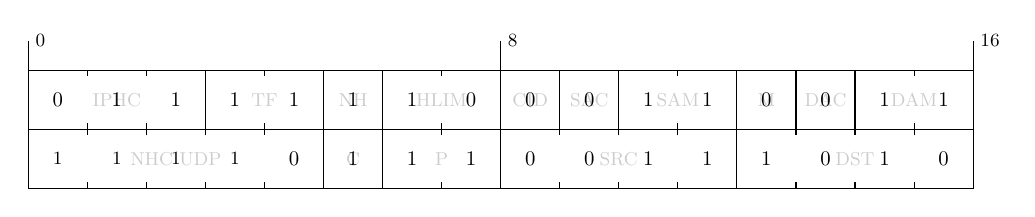
\begin{tikzpicture}[scale=0.75, every node/.append style={scale=0.75}]
		%IPHC
		\draw (0,0) rectangle (16,2);
		\draw (0,1) -- (16,1);
		\draw (0,2) -- ++(0,0.5) node[right] {\small 0};
		\draw (8,2) -- ++(0,0.5) node[right] {\small 8};
		\draw (16,2) -- ++(0,0.5) node[right] {\small 16};

		\foreach \x in {1,2,...,15}{
			\draw (\x,2) -- ++(0,-0.1);
			\draw (\x,1) -- ++(0,0.1);
			\draw (\x,1) -- ++(0,-0.1);
			\draw (\x,0) -- ++(0,0.1);
		}

		\draw (3,1) -- ++(0,1);
		\node at (1.5, 1.5) {\color{black!20}\small IPHC};
		\node at (0.5, 1.5) {0};
		\node at (1.5, 1.5) {1};
		\node at (2.5, 1.5) {1};

		\draw (5,1) -- ++(0,1);
		\node at (4, 1.5) {\color{black!20}\small TF};
		\node at (3.5, 1.5) {1};
		\node at (4.5, 1.5) {1};

		\draw (6,1) -- ++(0,1);
		\node at (5.5, 1.5) {\color{black!20} \small NH};
		\node at (5.5, 1.5) {1};

		\draw (8,1) -- ++(0,1);
		\node at (7, 1.5) {\color{black!20} \small HLIM};
		\node at (6.5, 1.5) {1};
		\node at (7.5, 1.5) {0};

		\draw (9,1) -- ++(0,1);
		\node at (8.5, 1.5) {\color{black!20} \small CID};
		\node at (8.5, 1.5) {0};

		\draw (10,1) -- ++(0,1);
		\node at (9.5, 1.5) {\color{black!20} \small SAC};
		\node at (9.5, 1.5) {0};

		\draw (12,1) -- ++(0,1);
		\node at (11, 1.5) {\color{black!20} \small SAM};
		\node at (10.5, 1.5) {1};
		\node at (11.5, 1.5) {1};

		\draw (13,1) -- ++(0,1);
		\node at (12.5, 1.5) {\color{black!20} \small M};
		\node at (12.5, 1.5) {0};

		\draw (14,1) -- ++(0,1);
		\node at (13.5, 1.5) {\color{black!20} \small DAC};
		\node at (13.5, 1.5) {0};

		\node at (15, 1.5) {\color{black!20} \small DAM};
		\node at (14.5, 1.5) {1};
		\node at (15.5, 1.5) {1};

		%UDP NHC
		\foreach \x in {0.5,1.5,...,3.5}{
			\node at (\x, 0.5) {\small 1};
		}

		\node at (2.5, 0.5) {\color{black!20} \small NHC UDP};

		\node at (4.5, 0.5) {0};
		\draw (5,0) -- ++(0,1);
		\node at (5.5, 0.5) {\color{black!20} \small C};
		\node at (5.5, 0.5) {1};
		\draw (6,0) -- ++(0,1);
		\node at (7, 0.5) {\color{black!20} \small P};
		\node at (6.5, 0.5) {1};
		\node at (7.5, 0.5) {1};
		\draw (8,0) -- ++(0,1);
		\node at (10,0.5) {\color{black!20} \small SRC};
		\node at (8.5, 0.5) {0};
		\node at (9.5, 0.5) {0};
		\node at (10.5, 0.5) {1};
		\node at (11.5, 0.5) {1};
		\draw (12,0) -- ++(0,1);
		\node at (14,0.5) {\color{black!20} \small DST};
		\node at (12.5, 0.5) {1};
		\node at (13.5, 0.5) {0};
		\node at (14.5, 0.5) {1};
		\node at (15.5, 0.5) {0};
		\draw (16,0) -- ++(0,1);
	\end{tikzpicture}
	\caption{Link-Local IPv6 an UDP header to IPHC example}
	\label{fig:6lo_example}
\end{figure}

\autoref{fig:6lo_example} depicts an optimal compression of a Link-Local IPv6 packet with UDP.
The Traffic-Class (TC) and Flow-Label (FL) field can be fully elided because they are zero.
All-zero TC and FL are a realistic scenario for Link-Local traffic and even for the most routed traffic.
The UDP Next-Header-Field can be elided because we can use Next-Header-Compression for UDP.
A Hop-Limit of 64 can be compressed with no in-line data added.
The IPv6 Source Address and destination address can be compressed to zero in-line data.
The Link-Local prefix can be fully elided, and the IID can be reconstructed from the Link-Layer address.
The UDP header is compressed by using the UDP Next Header Compression.
The source and destination ports are chosen in a way that they can be efficiently compressed to a single byte.
This efficient compression works for addresses of form 0xf0bX, where the last nibble can be chosen.
The checksum is elided in this example.
It can be elided if the link-layer already has a mechanism for checking the correctness of the data.

Efficient compression heavily depends on the IPv6 address and ports used.
To have an efficient compression, the IDD should be derived from the Link-Layer address,
and the prefix should either be link-local, or a context should be distributed among all nodes.
RFC6282 does not define how to distribute the IPHC context; neither does this work do.
Applications that are aware of the fact that IPHC is used,
should use ports from 0xf0b0 to 0xf0bf to allow efficient UDP Next Header Compression.

\FloatBarrier

\section{Zephyr}
\label{sec:zephyr}
Zephyr is a Real-Time Operating System (RTOS) launched by Intel and now hosted by the Linux Foundation as the Zephyrproject.
The kernel is derived from WindRiver's Rocket kernel, and the Zephyr project source code is publicly available on GitHub under the Appache 2 license.
The development is community and industry-driven with vendor-neutral governance.
Major System on Chip (SoC) vendors are members of the project and provide funding.
Zephyr is designed for small scale connected devices, but it can also run on an x68 application processor.
Is supports various architectures like ARM, x64, ARC, RISC-V, and Xtensa.
For each architecture, a set of SoCs and development boards are supported.

\FloatBarrier

\section{Zephyr Network Stack}
\label{sec:network_stack}
Zephyr has a native IPv4 and IPv6 network stack built-in. The stack is authored and maintained by the Zephyr community.
It supports TCP and UDP transport and all ICMP packets required by the IP standards.
The interface provided to the user is a POSIX Sockets API.
Currently the following Link-Layers are supported:

\begin{itemize}
	\item Ethernet
	\item 6LoWPAN (IEEE 802.15.4)
	\item IPSP (Bluetooth Low Energy)
	\item 6LoCAN (Controller Area Network), as an outcome of this work
\end{itemize}

\begin{figure}[htp]
	\begin{center}
	\begin{tikzpicture}[
		scale=0.7,
		every node/.append style={scale=0.7},
		layers/.style={
			align=left,
			fill=blue!5,
			rectangle,
			draw=blue!5,
			node distance=0.2cm},
		layers_dark/.style={
			draw=black,
			fill=blue!15,
			rectangle,
			node distance=0.2cm},
		layer_rot/.style={
			draw=black,
			fill=blue!15,
			rectangle},
		instance/.style={
			draw=black,
			rounded corners=0.05cm,
			fill=blue!15,
			rectangle, 
			minimum width=2cm,
			minimum height=1cm,
			align=center,
			font=\small},
		instance_wide/.style={
			draw=black,
			rounded corners=0.05cm,
			fill=blue!15,
			rectangle, 
			minimum width=4cm,
			minimum height=1cm,
			align=center,
			font=\small}
		]

		%App
		\node (app)[layers_dark, draw=blue!15, node distance=0cm, minimum width = 9.8cm, minimum height = 1.5cm] {Networking Application};
		\node (appbare)[layers_dark, draw=blue!15, node distance=0cm, right = of app.north east, anchor=north west, xshift=0cm, minimum width = 2.2cm, minimum height=5.8cm] {};
		\draw (app.north west) -- (appbare.north east) -- (appbare.south east) -- (appbare.south west) -- (app.south east) -- (app.south west) -- (app.north west);
	
		%Application Protocols
		\node (appprot)[layers,below = of app.south west,anchor=north west, minimum width=9.6cm, text width = 9.1cm, minimum height = 4cm, text depth=3cm] {Application Protocols};
		\foreach \approtocol/\x/\y in {CoAP/-2.5/0.75, LWM2M/2.5/0.75, MQTT/-2.5/-0.5, etc./2.5/-0.5}{
			\node at ($(appprot) + (\x cm, \y cm -0.5 cm)$) [instance_wide] {\approtocol};
		}
		
		%Sockets API
		\node (sockets)[layers_dark, below = of appprot.south west,anchor=north west, minimum width = 10.8cm, minimum height = 1cm] {Sockets API};

		%Net-context
		\node (netctx)[layers_dark, below = of sockets.south west,anchor=north west, minimum width = 10.8cm, minimum height = 1cm] {Net-Context API};
	
		%Transport-Layer Protocols
		\node (transp)[layers,below = of netctx.south west,anchor=north west, minimum width = 9.6cm, text width = 9.1cm, minimum height = 4cm, text depth = 3cm] {Transport-Layer Protocols};
		\foreach \tansport/\x/\y in {TCP/-2.5/0.75, UDP/2.5/0.75, ICMPv4/-2.5/-0.5, ICMPv6/2.5/-0.5}{
			\node (\tansport) at ($(transp) + (\x cm, \y cm -0.5 cm)$) [instance_wide] {\tansport};
		}

		%Networking Protocols
		\node (netw)[layers,below = of transp.south west,anchor=north west, minimum width=9.6cm, text width=9.1cm, minimum height = 2.5cm, text depth = 1.5cm] {Networking Protocols};
		\foreach \network/\x in {IPv4/-2.5, IPv6/2.5}{
			\node (\network) at ($(netw) + (\x cm, -0.5 cm)$) [instance_wide] {\network};
		}

		\node (netcore)[layers_dark, below = of netw.south west,anchor=north west, minimum width = 10.8cm, minimum height = 1cm] {Network Core};

		%Interface Abstraction
		\node (interf)[layers_dark, below = of netcore.south west,anchor=north west, minimum width = 10.8cm, minimum height = 1cm] {Network Interface Abstraction Layer};

		%Non-IP Sockets
		\node at ($(netctx)!0.5!(netcore) + (4.9cm ,0)$) [layer_rot, rotate=90, minimum width=6.8cm, minimum height=1cm] {Non-IP Sockets};

		%Link-Layer
		\node (linklayer)[layers, below = of interf.south west,anchor=north west, minimum width = 10.8cm, text width = 10.3cm, minimum height = 2.5cm, text depth = 1.5cm] {Link-Layer Technologies};
		\foreach \linklayer/\x in {Ethernet/-4, 6LoWPAN/-1.25, 6LoCAN/1.25, IPSP/4}{
			\node (\linklayer) at ($(linklayer) + (\x cm, -0.5 cm)$) [instance] {\linklayer};
		}
		
		%Network drivers
		\node (net_drivers)[layers, below = of linklayer.south west,anchor=north west, minimum width = 12cm, text width = 11.5cm, minimum height = 3cm, text depth = 2cm] {Network Device Drivers};
		\foreach \driver/\x in {Ethernet/-4.5, CAN/-1.5, 802.15.4/1.5, Other/4.5}{
			\foreach \inst in {0.3,0.2,0.1}{
				\node at ($(net_drivers) + (\x cm - \inst cm, -0.5 cm + \inst cm)$) [instance] {};
			}
			\node (\driver)  at ($(net_drivers) + (\x cm, -0.5 cm)$) [instance] {\driver \\ drivers};
		}

		%Network Management API
		\node at ($(appbare.south east)!0.5!(net_drivers.north east) + (-0.5cm ,0)$) [layer_rot, rotate=90, minimum width=14.8cm, minimum height=1cm] {Network Management API};
	\end{tikzpicture}
	\caption{Zephyr Network Stack 6LoCAN RX example}
	\label{fig:zephyr_net_satck}
	\end{center}
\end{figure}


\autoref{fig:zephyr_net_satck} depicts an overview of the Zephyr stack.
On the bottom, there are the implementations of the low-level network device drivers.
They are responsible for handling the interrupts, sending, and receiving raw data.

The next layer is the Link-Layer Technologies Layer.
This layer takes care of the Link-Layer headers, and in the case of 6lo Technologies, performs fragmentation, reassembly, IPv6 header-compression, and uncompression.

The Network Core Layer is kind of a dispatcher for packets.
It accepts raw packets from the network and put them into the networking working queues, depending on the packet priority.
This layer is the boundary between the driver context, that could possibly be an interrupt, and networking context.
The networking context consists of multiple work-queue threads for receiving and sending.
The work-queue threads have different priorities, to support traffic classification by priority.
The number of threads can be chosen by a configuration option.

The Network Interface Abstraction Layer defines a common API for Link-Layer implementations,
handles the IP addresses of the interface and provides a generic way to read the Link-Layer addresses.

The Networking Protocols Layer parses the IP headers, checks the addresses, and decides if the packet is addressed to this node or should be discarded.
It also parses the next header and invokes the corresponding transport protocol.

The Transport-Layer Protocols Layer parses and validates the transport layer protocol header.
In the case of ICMP, the packets are handled by this layer, while TCP and UDP packets are handed over to the Net-Context API by the IP layer.

The Net-Context API layer checks for registered handlers and if a handler is found, forwards it to them.
The Sockets API registers the handlers, that takes the packet from the Net-Context and forwards it to the user application.
The Sockets API follows the POSIX \cite{posix} BSD sockets API standard.
